% Ejemplo del uso de la template para escribir tesis/memorias de la Universidad Diego Portales.
%
% Eviar bugs a: Adín Ramírez, adin.ramirez (at) mail.udp.cl

% Puede generar borradores si omite la opción "final" de la clase.
% \documentclass{udpthesis}
\documentclass[final]{udpthesis}

% Establecemos el sistema para uso del español
% Babel ya esta cargado dentro de updthesis
\usepackage[T1]{fontenc}%    output
\usepackage[utf8]{inputenc}% input
\usepackage{lmodern}
\usepackage{listings}
\usepackage{tikz}
\usepackage{pgfplots} % fuer plots

\usepackage[external]{forest}


% Leyendas
\usepackage[font=footnotesize,labelfont=bf,labelsep=period]{caption}

% Agregue acá otros paquetes que le sean de utilidad

\usepackage{amsmath}	% Matemáticas
\usepackage{graphicx}	% Gráficos
\usepackage[font=footnotesize,labelformat=simple]{subfig}

% Cambiamos el formato de las leyendas: finalizan en punto, y en negrita.
\captionsetup{labelsep=period,labelfont=bf}
% Habilitamos el uso de paréntesis al citar las figuras con subfiguras dentro, e.g., Fig. 1(a)
\renewcommand\thesubfigure{(\alph{subfigure})}
\renewcommand\thesubtable{(\alph{subtable})}
\newcommand{\subfigureautorefname}{\figureautorefname}


\lstset{
 % language=[LaTeX]TeX,
 breaklines=true,
 basicstyle=\tt\scriptsize,
 keywordstyle=\color{blue},
 identifierstyle=\color{black},
 commentstyle=\color{green!40!black},
 % frame 
 frame=tb,
 captionpos=t,
 xleftmargin=1em,
 numbersep=0.3em,
 % numbers=left,
 framexleftmargin=1.1em,
 framexrightmargin=0pt,
 % additional letters for accents in spanish
 literate=%
   {á}{{\'{a}}}1
   {é}{{\'{e}}}1
   {í}{{\'{i}}}1
   {ó}{{\'{o}}}1
   {ú}{{\'{u}}}1
   {ñ}{{\~{n}}}1
   {Ñ}{{\~{N}}}1
}


% Código
% Para generar código fuente usar listings.sty
%\usepackage{listings}
%\usepackage{tikz}
%\lstset{
%  language=[LaTeX]TeX,
%  breaklines=true,
%  basicstyle=\tt\scriptsize,
%  keywordstyle=\color{blue},
%  identifierstyle=\color{magenta},
%  commentstyle=\color{green!40!black},
%  % frame 
%  frame=tb,
%  captionpos=t,
%  xleftmargin=1em,
%  numbersep=0.3em,
%  numbers=left,
%  framexleftmargin=1.1em,
%  framexrightmargin=0pt,
%  % additional letters for accents in spanish
%  literate=%
%    {á}{{\'{a}}}1
%    {é}{{\'{e}}}1
%    {í}{{\'{i}}}1
%    {ó}{{\'{o}}}1
%    {ú}{{\'{u}}}1
%    {ñ}{{\~{n}}}1
%    {Ñ}{{\~{N}}}1
%}
%
%\renewcommand{\lstlistingname}{Código}% Listing -> Código
%\DeclareCaptionFormat{listing}{\rule{\dimexpr\linewidth\relax}{0.4pt}\par\vskip1pt#1#2#3}
%\captionsetup[lstlisting]{format=listing,singlelinecheck=false, margin=0pt,position=bottom}

% O para generar algoritmos en pseudocódigo usar algpseudocode.sty
%\usepackage{algorithm}
%\usepackage{algpseudocode}
\usepackage{algpseudocode}
%\makeatletter
%\renewcommand{\ALG@name}{Algoritmo}% Algorithm -> Algoritmo
%\makeatother
%\captionsetup[algorithm]{font=footnotesize,labelsep=period}
% Referencias (este paquete ordena y comprime las referencias)
\usepackage{cite}


\usepackage{blindtext}



\udptheme{EIT}


\begin{document}

\frontmatter		%% Inicio de la portada



% Título del tema (no más de 12 palabras)
\title{Modelo de Predicción Secuencial de Web Access Log basado en Algoritmos de Compresión y Machine Learning}
% para precisar aún más su tema, use un subtítulo
%\subtitle{Subtítulo explicativo del tema}


\author{Jaime Guzmán}
\email{mail@jguzman.cl}




\date{2015}

% Profesor guía
\professor{Adin Ramirez}
% Comité
\committee{Francisco Claude}{Darth Vader}

% Dedicatoria
\dedicatory{Utilice un par de oraciones para dedicar su tesis, o una frase de alguién importante.}

% Agradecimientos
\acknowledgment{Nota redactada sobriamente en la cual se agradece a quienes han colaborado en la elaboración del trabajo. No puede exceder más de una página.}

% Abstrat en inglés
\abstract{%<- evita nueva linea en el abstract
Abstract is the summary in english of the subject your are presenting in this thesis. Should not exceed one page.
}

% Resumen
\resumen{
%<- evita nueva linea en el resumen 
%El resumen no debe contener menos de 100 palabras ni mas de 300 palabras.

El siguiente documento comprende el estudio y creación de un modelo híbrido entre Machine Learning y Algoritmos de tipo Lossless Data Compression. Internet crece cada día y los datos crecen en volúmenes del orden de los Terabytes, por lo cual es de interés usar técnicas de compresión para realizar  procesamiento a mayor escala de información con la menor cantidad de recursos posibles.

Hoy existe variadas tipos de web, redes sociales, microbloging, web informativas, etc. El contenido proporcionado a los usuarios finales  ya no es estático y esto permite que los mismo puedan generar, aportar, modificar contenido, dado  esto la ingeniería ofrece para construir web esta en constante evolución lo que ha ayudado a generar mas recursos para poder desarrollarla. Muchas de estas nuevas tecnologías han permitido entregar una mejor experiencia al momento de navegar, aún cuando se ha creado un gran avance sobre el mismo esto no ha permitido crear Web que sean por sí mismas inteligente y puedan ir anticipando su comportamiento, para por ejemplo; disminuir la latencia desde que se abre una web ya visitada o desde que se navega dentro de un sitio con alta demanda; también desde el punto de vista de la arquitectura como servicio que las hospedan no se ha visto abarcada, dando un aspecto económico a los recursos utilizados. Si bien el crecimiento de los recursos de almacenamiento en la nube se encuentran un apogeo, las redes no crecen a la misma velocidad. 

Este trabajo busca predecir la siguiente página que un usuario pueda acceder dentro en una web. Usando técnicas de entrenamiento y algoritmo de compresión. Con este propósito se trabajará para crear un modelo predictivo que use estas dos áreas.
}


\makecover			% Generamos la portada

% Indices y listas
\tableofcontents	% tabla de contenido
\listoftables		%    índice de tablas
\listoffigures		%   índice de figuras
% puede agregar otras listas o índices acá de ser necesario



% Inicio del contenido
\mainmatter


\chapter[Introducción]{Introducción}
\label{ch:intro}

%chacharara
{
  El área de las ciencias de la computación que se encarga de estudiar todos los datos de maneras en que entregue información relevante, para poder ser estudiada es la Minería de Datos. Hoy en día esta área toma mucha relevancia al encontrarnos en una auge de la información generada por usuarios, redes sociales y variadas plataformas, podemos mencionar que esta es una de las razones para poder requerir disponer de herramientas de analisis que nos permitan saber como se comporta usuarios sobre una web, conocer la frecuencia en que se accede a un recurso en internet, etc.
  
  Sea el caso que entre una conexión cliente-servidor, una gran cantidad de servicios proporcionan datos de acccesos de los usuarios que acceden, sobre estos mismos existe se puede realizar un estudio sobre como predecir cual es la siguiente página que van a visitar.
  }

% Normalmente se ocupa muchos algorimot de maquinas de aprendizaje para poder hacer predicciones en variadas areas,

% Nuestro intere es hacer que las rpecicciones sean modeladas por un compresaor de datos basado en Lempel ziv



%%%%%%%%%%
% Uno de los interes en poder crear un un aplicación de ambas areas es la convergenia de las areas en la cual un proceso de aprendizaje ó predicción secuencial se puede usar con ML y Compress data
% Cuando se hace el pio train se hace un entrenamiento de modelo lo que resulta ser es que genera el arbol que es un trie de LZ que será el predicto
% Una función de predición implementada con MLIB y PIO sería predict () en scala




%%%%%%% CONTEXTO PRELIMINAR 
\section{Contexto Preliminar} \label{sec:preliminar}

  La Web crece constantemente y por ende su infraestructura, también la información que podemos obtener de los  usuarios y  concurrencia de los sistemas, la cual para usuarios finales se traduce en latencia y una mejor o peor experiencia de usuario. Paralelamente se suma un costo exponencial de recursos tanto en tecnologías de desarrollo como servicio que no son optimizados para poder dar una experiencia de usuario con calidad de servicio. Podemos reflexionar, entonces, que el no tener mayores recursos mejorará el rendimiento ni tampoco será lo óptimo para dar una calidad de servicio web, ya que el ancho de banda de Internet no crecerá a la misma proporción.
   
  Adicionalmente, las tecnologías para la creación de web dinámicas e asíncronas han evolucionado a favor de traspasar la carga cliente.
  Hoy en día ya se poseen leguanjes y framework que disminuyen considerablemente la carga de un servidor, por lo cual, un buen servicio web es proveer una balanceada carga dentro del cliente y el servidor, pero cuando se poseen un volumen de datos grandes es requerido tomar decisiones que los recursos y lenguajes no cubren, es ahí el interés de dar inteligencia a los servicios web.

  Predecir los futuros accesos que un usuario tendrá en una determinada web. Entendiendo que la manera en que un usuario navega es su comportamiento registrado en una web, y que se puede analizar, estudiar y registrar mediante \emph{Web Access Log} y a los cuales se puede hacer una minería de datos, Web Usage Minning. El por qué de hacer minería de datos es que cada día la web genera un innumerable cantidad de datos, por lo cual usar un algoritmo que se puedan operan comprimidos presenta un interés ya que además de disminuir el espacio físico o recursos utilizados, este se puede usar como un algoritmo de predicción y trabajar con una mayor cantidad de datos.
  
  Los registros de accesos de manera procesada o pre-procesada, ayudaría a ingenieros de desarrollo web y diseñadores, como a  usuarios finales a tener una experiencia de usuario mejor, disminuyendo por ejemplo la latencia en respuestas por parte de cada petición que realizan.
  
  Hoy en día, las web no pueden ser simplemente dinámicas en contenidos, debe poseer una adaptabilidad a la demanda del usuario o proveer información que permita adaptarse a los eventos, por lo tanto, es de interés el profundizar en este tópico.

  El interés en hacer un estudio sobre esto es poder hacer integraciones en áreas como compresión y la áreas que se dedican a completamente a hacer estudios sobre maquinas de aprendizaje. De por sí solas cada una se abordado independientemente lo cual es un interés converge en un problema en común que se puede resolver de manera eficiente.

  Durante este trabajo se usarán técnicas de compresión de datos, se utilizará una infraestructura y patrón de implementación para modelos de Machine Learning. Adicionalmente toda la experimentación se llevará acabo disponibilizando los algoritmos y modelos como servicio REST, el cual se explicará mas adelante, ya mencionado lo anterior este trabajo es implementable en áreas productivas las cuales pueden presentar interés.

  Definiremos que un usuarios es un la que se conecta a un servicio web, estos pueden ser paginas web informativas, redes sociales, etc. Este usuario establece una conexión directa con una pagina al momento de realizar esta operación, es posible almacenar datos los cuales vamos a llamar "access log" ó registros de accesos, durante el texto se mantendrán las referencias en ingles.

  Un ejemplo de access log podría ser el siguiente:


\begin{verbatim}
  172.31.33.116 - - [26/Nov/2015:00:12:11 +0000] "GET /wp-content/themes/corridacuprum/images/cuprum-footer.png HTTP/1.1" 200 4447 "http://virtual.corridacuprumteleton.cl/?utm_source=masterbase&utm_medium=mail2&utm_campaign=corrida-cuprum-teleton&utm_campaign=8474:%20%23!nombre!%23%2c+PARTICIPA+EN+LA+CORRIDA+VIRTUAL+Y+APOYA++A+LA+TELETON&utm_source=MasterBase%20CUPRUM&utm_medium=email&utm_content=2&utm_term=none" "Mozilla/5.0 (Linux; Android 5.1.1; SAMSUNG SM-G920I Build/LMY47X) AppleWebKit/537.36 (KHTML, like Gecko) SamsungBrowser/3.2 Chrome/38.0.2125.102 Mobile Safari/537.36"
  172.31.33.116 - - [26/Nov/2015:00:12:12 +0000] "GET /wp-content/themes/corridacuprum/images/principal-footer.png HTTP/1.1" 200 1784 "http://virtual.corridacuprumteleton.cl/?utm_source=masterbase&utm_medium=mail2&utm_campaign=corrida-cuprum-teleton&utm_campaign=8474:%20%23!nombre!%23%2c+PARTICIPA+EN+LA+CORRIDA+VIRTUAL+Y+APOYA++A+LA+TELETON&utm_source=MasterBase%20CUPRUM&utm_medium=email&utm_content=2&utm_term=none" "Mozilla/5.0 (Linux; Android 5.1.1; SAMSUNG SM-G920I Build/LMY47X) AppleWebKit/537.36 (KHTML, like Gecko) SamsungBrowser/3.2 Chrome/38.0.2125.102 Mobile Safari/537.36"
  172.31.33.116 - - [26/Nov/2015:00:12:12 +0000] "GET /wp-content/themes/corridacuprum/images/main.png HTTP/1.1" 200 179333 "http://virtual.corridacuprumteleton.cl/wp-content/themes/corridacuprum/style.css?ver=3.8.1" "Mozilla/5.0 (Linux; Android 5.1.1; SAMSUNG SM-G920I Build/LMY47X) AppleWebKit/537.36 (KHTML, like Gecko) SamsungBrowser/3.2 Chrome/38.0.2125.102 Mobile Safari/537.36"
  172.31.33.116 - - [26/Nov/2015:00:12:12 +0000] "GET /wp-content/themes/corridacuprum/fonts/akzidenzgrotesk-eb.woff2 HTTP/1.1" 200 24660 "http://virtual.corridacuprumteleton.cl/wp-content/themes/corridacuprum/style.css?ver=3.8.1" "Mozilla/5.0 (Linux; Android 5.1.1; SAMSUNG SM-G920I Build/LMY47X) AppleWebKit/537.36 (KHTML, like Gecko) SamsungBrowser/3.2 Chrome/38.0.2125.102 Mobile Safari/537.36"
  172.31.33.116 - - [26/Nov/2015:00:12:12 +0000] "GET /wp-content/themes/corridacuprum/fonts/akzidenzgrotesk-mc.woff2 HTTP/1.1" 200 24604 "http://virtual.corridacuprumteleton.cl/wp-content/themes/corridacuprum/style.css?ver=3.8.1" "Mozilla/5.0 (Linux; Android 5.1.1; SAMSUNG SM-G920I Build/LMY47X) AppleWebKit/537.36 (KHTML, like Gecko) SamsungBrowser/3.2 Chrome/38.0.2125.102 Mobile Safari/537.36"
  172.31.33.116 - - [26/Nov/2015:00:12:12 +0000] "GET /wp-content/themes/corridacuprum/images/lines-left.png HTTP/1.1" 200 4860 "http://virtual.corridacuprumteleton.cl/wp-content/themes/corridacuprum/style.css?ver=3.8.1" "Mozilla/5.0 (Linux; Android 5.1.1; SAMSUNG SM-G920I Build/LMY47X) AppleWebKit/537.36 (KHTML, like Gecko) SamsungBrowser/3.2 Chrome/38.0.2125.102 Mobile Safari/537.36"
  172.31.33.116 - - [26/Nov/2015:00:12:12 +0000] "GET /wp-content/themes/corridacuprum/images/lines-right.png HTTP/1.1" 200 4841 "http://virtual.corridacuprumteleton.cl/wp-content/themes/corridacuprum/style.css?ver=3.8.1" "Mozilla/5.0 (Linux; Android 5.1.1; SAMSUNG SM-G920I Build/LMY47X) AppleWebKit/537.36 (KHTML, like Gecko) SamsungBrowser/3.2 Chrome/38.0.2125.102 Mobile Safari/537.36"
  	
  \end{verbatim}

  El ejemplo anterior nos da mucha información interesante como la IP desde donde se conecta, el tipo de navegador, el dispositivo si es un telefono inteligente o un navegador de escritorio, la fecha en que se realizo el acceso y también lo mas relevante el destino del usuario.








% @TODO: SEGUIR TRABAJANDO EN ESTA BREVE INTRODUCCION
%En este tema convergen tres áreas, por un lado existe trabajo para crear estructuras eficientes para predicciones basadas en algoritmos de compresión, como es en el caso de~\cite{Claude2014}, y, por otro lado, el uso de algoritmos de aprendizaje para realizar clustering y predecir el comportamiento basado en el mismo contenido o en la distancia del contenido que visita el usuario actual al contenido clusterizado, como es el caso de ~\cite{Poornalatha2012}, inclusive se han utilizado modelos de Markov en ~\cite{Dongshan2002}  para poder modelar el comportamiento de la web.
%La tercera área son los Sistemas de Recomendación, la cual en este proyecto no se tocará pero si se mencionará el enfoque práctico que presenta área como un foco de múltiples implementaciones. 







%Algoritmos como serivcio
\section{Algoritmos como servicio web }

	Los avances en el desarrollo de nuevas tecnología que brinden mejores experiencias en su uso del día a día, deriva en cómo podemos llevar varios escenarios idealizados a implementaciones empresariales reales. Es bastante común encontrar librerías que son bastante útiles para hacer Minería de Datos, Clustering y muchas operaciones que pueden recurrir en cálculos muy complejos pero no se pueden ofrecer como servicio. Ya en auge de las infraestructuras Cloud, la capacidad de computo que se puede alcanzar no es un problema a lo que antes se enfrenta un Cientista de Datos.


	Una API es un interfaz de programación de Aplicaciones que nos permiten intermediar el Servicio A con el Servicio B. Respectivamente A puede ser el proveedor y B el Demandante de servicios. Si quisiéramos analizar datos que se encuentran dentro de un servidor especifico, estos se podrían consumir por esta interfaz. Existen variados clientes que nos permiten ayudar a esta comunicación, incluso se pueden utilizar por una terminal de Unix la cual es posible que mediante el programa $curl$, el cual permita dialogar con un determinado servicio web.
	
	Ya se dispone de infraestructura como servicio, software como servicio, plataformas como servicios. Dado lo anterior ofrecer estos algoritmos para hacer que las soluciones de desarrollo den valor agregado a la experiencia requerida por el usuario. Así es que hemos decidido utilizar una librería y framework que nos de esta posibilidad. Ofrecer algoritmos a la industria como un servicio que ayuda de manera inteligente y multiplataforma que es el caso de una API. 
	
	Todas las ventajas de este patrón son heredados de las características que ofrece una API, interoperabilidad, evitar problemas de Infraestructura, Resiliencia de Datos, Persistencia de Datos, Análisis y Procesamiento sin afectar un curso operacional de una aplicación. Un ejemplo claro de esto es el análisis de datos en sistemas legados los cuales en plan de mejoras, no poseen la compatibilidad para poder realizarlo. Por otro lado, los algoritmos de compresión o algoritmos de Machine Learning tienden ocupar recursos y este hecho pueden ser la razón para no implementarlos. 
	
	
	
	




%introducción a las Prediccion


\section{Predicción }

  	
En esta sección se presenta formalmente el ambiente de desarrollo que se utilizará durante este trabajo. \emph{PredictionIO} es un servidor de \emph{Machine Learning} de código abierto para Científico de Datos y Desarrolladores que permite crear motores de predicción para aplicaciones en producción, con un bajo tiempo de entrenamiento y despliegue. Principalmente está construido en \emph{Apache Spark, HBase} y \emph{Spray}. 

Este ambiente de trabajo se encuentra en un maduración estable y constante que permite tanto disponer servidores con motores predictivos, como también toda una infraestructura distribuida para hacer que complejos algoritmos sean utilizados para solucionar problemas reales.



% PIO, tiene practicamente todo armadao, ello no hicieron nada nuevo ... solo juntaron  todo...



% He estado investigando y revisando documentación, Yelp, Skype, Hubot de github y otras implementaciones tienen usando prediction.io




% La otra opción es meterle a este "DASE" un algoritmo  que mezcle una representación de cadenas de markov mezclado con LZ78. no se en que punto mezclarlo en el diccionario, o la verdad es como hacer el compresor sea "mas inteligente", encontré un papaer que te adjunto en el cual usan lz78 y lzw, esta interesante ya que le hacen un acercamiento mas al tema de de ser un predictor online.


% Ahora entiendo que la cadenas de markov son y se han ocupado para las predicciones, pero no veo la necesidad de ocuparlas mayormente. Adin me inisiste en que le de una vuelta.... pero mi sensación  es que tengo separada las ideas en dos extremos. 

% Ya revise Suffix Tree para predicciones LZ77 y LZW, también PPM y HMM.

 
 



\subsection{Arquitectura DASE}


Un motor de predicción es un tipo de proceso en \emph{Machine Learning}. Siguiendo una arquitectura de tipo \emph{DASE}, contendríamos los siguientes componentes.



\begin{itemize}

  \item\label{dase-datasource} \textbf{ $[D]$ Data Source y Data Preparator}. Los Data Source leen la data desde la entrada original y la transforman en un formato deseado para hacer análisis de estos. En cambio \emph{Data Preparator} pre-procesa la información y la reenvía a los algoritmos para   hacer el modelo de entrenamiento.


  \item\label{dase-algoritmo} \textbf{ $[A]$ Algoritmo}. Los componentes de \emph{PredictionIO}, dada sus librerías incluyen algoritmos de \emph{Machine Learning}, estos, pueden ser provistos por \emph{Apache Spark} o se pueden incluir algoritmos propios como también de terceros.
    Adicionalmente a los algoritmos podemos asignarle parámetros, para determinar como debiese ser construido el motor ó si es requerido para un cierto algoritmo.



  \item\label{dase-servicio} \textbf{ $[S]$ Servicio}. El componente servicio toma las consultas ó \emph{queries} de predicción y retorna los resultados, en nuestro modelo propuesto en la etapa experimental veremos el siguiente símbolo de una secuencia. 
  Si el motor de predicción tiene múltiples algoritmos, combinará los resultados en uno. Adicionalmente, la lógica específica de negocios puede ser añadida para especificar aún más el resultado final. 
 
  \item\label{dase-eval} \textbf{ $[E]$ Evaluación de Métricas}.
Las métricas de evaluación cuantifican la precisión de la predicción con una puntuación numérica. Puede ser utilizado para la comparación de algoritmos o ajustes de los parámetros del algoritmo.
\end{itemize}




  \tikzstyle{decision} = [diamond, draw,text width=4.5em, text badly centered, node distance=2.5cm, inner sep=0pt]
  \tikzstyle{block} = [rectangle, draw,text width=5em, text centered, rounded corners, minimum height=4em]
  \tikzstyle{line} = [draw, very thick, color=black!50, -latex']
  \tikzstyle{cloud} = [draw, ellipse, node distance=2.5cm,
  minimum height=2em]


\begin{figure}[t]
	\centering	
	\resizebox{0.8\textwidth}{!}{% <------ Don't forget this %
	
		\begin{tikzpicture}[scale=1, node distance = 2.5cm, auto]
		% Place nodes
		
		\node [block] (init) {Data de la Aplicación};
		\draw [color=gray,thick](1.3,1) rectangle (11.2,-3.5);    
		
		\node [block,right of=init] 		  (datasource) {Data Source};
		\node [block,right of=datasource]     (datapreparator) {Data Preparator};
		\node [block,right of=datapreparator] (alg1) {Algoritmo };
		\node [block,right of=alg1] 		  (serving) {Serving};
		\node [block,below of=serving] 		  (evalmetric) {Evaluación Métrica};
		\node [block,right of=serving] 		  (resultpredict) {Resultado Predicción};
		\node [block,below of=resultpredict]  (resulteval) {Resultado Evaluación};
		
		\path [line] (init) -- (datasource);
		\path [line] (datasource) -- (datapreparator);
		\path [line] (datapreparator) -- (alg1);
		\path [line] (alg1) -- (serving);
		\path [line] (serving) -- (evalmetric);
		\path [line] (serving) -- (resultpredict);
		\path [line] (evalmetric) -- (resulteval);    
		
		\end{tikzpicture}
	}
	\caption{Diagrama de componentes Arquitectura DASE.}
	\label{fig:arquitectura-dase}
\end{figure}



\vspace{1cm}

\emph{PredictionIO} ayuda a tener componentes muy modulares, las que ya hemos descrito como  arquitectura \emph{DASE}(\ref{fig:arquitectura-dase})  que puede construir modelos de predicción de manera sencilla. También poder integrarlos con gran facilidad a cualquier sistema o plataforma, por ejemplo, es posible elegir cual de todos los componentes se podrá desplegar al momento de crear un \emph{Engine} (Motor de Predicción.)



\vspace{1cm}
\subsection{Despliegue de motor de predicción}

  Un \emph{Motor de predicción} pone todos los componentes del diseño de arquitectura \emph{DASE} en un estado especifico de despliegue 
  \begin{enumerate}
  		\setlength{\itemsep}{1pt}
  		\setlength{\parskip}{0pt}
  		\setlength{\parsep}{0pt}
    \item Data Source
    \item Data Preparator
    \item Uno o más Algoritmos generadores de Modelos
    \item Un Servicio 
  \end{enumerate}

  Si se especifica más de un algoritmo, cada uno de los resultados de los modelos de predicción se entregará para ser consumido por cualquier cliente.
  Cada \emph{motor de predicción} procesa los datos y construye un modelos de forma independiente. Por lo tanto, todos los motores de predicción que usaremos sirven a su propio conjunto de resultados. Por ejemplo, se puede desplegar dos \emph{motores predictivos} para una aplicación móvil: uno para recomendar noticias a los usuarios y otro para sugerir nuevos amigos a los usuarios.


\vspace{1cm}
\subsection{Evaluación del motor de predicción }

  Para evaluar el \emph{Accuracy} de un motor de predicción, se debe especificar la métrica seleccionad cuando se corre el motor de evaluación, en los capítulos experimentales se verá como se generan métricas y como se desempeña esta métrica para ser evaluada.











\subsection{Modelamiento de eventos}

%https://docs.prediction.io/datacollection/eventmodel/




  El modelamiento de eventos es fundamental para un predictor \emph{online}, el hecho de poder llevar un vector con ciertas propiedades característica\footnote{Característica de un cierto dataset para entrenar.} de una representación vectorial del mundo del \emph{Machine Learning} a un modelamiento secuencial, es en realidad el modelamiento que se debe realizar de como  tener las muestras de datos para generar \emph{Resilient Distributed Dataset} (RDD) que son un parte principal de nuestro ambiente de trabajo con \emph{PredictionIO} para poder acceder posterior o inmediatamente. 

  Un evento lo definiremos como entidad que nos permite dar una representación temporalizada de información que será procesada por un motor de predicción. Analizaremos los eventos que un usuarios realiza para poder acceder a una web. Adicionalmente cuando cada usuario ingresa a una web automáticamente este genera una sesión, desde que que llega hasta que abandona la web.

  Usaremos un \emph{dataset} con información que esta totalmente depurada y recuperada de los access log (provista por Claude \etal~\cite{Claude2014}), los cuales a efectos de temporalidad solo nos interesa conocer la secuencialidad de estos accesos.
  


%Poner algo mas matematico.
% EVENT API 
% https://docs.prediction.io/datacollection/eventapi/

  El modelamiento que realizaremos contempla los siguientes campos :
  \begin{itemize}
    		\setlength{\itemsep}{1pt}
    		\setlength{\parskip}{0pt}
    		\setlength{\parsep}{0pt}
      \item Tipo de Evento: Visitar
      \item Entidad que ejecuta el evento: Usuario
      \item Propiedades:
          \begin{enumerate}
          		\setlength{\itemsep}{1pt}
          		\setlength{\parskip}{0pt}
          		\setlength{\parsep}{0pt}
            \item Página actual
            \item Página siguiente
            \item Cierre de Sesión
          \end{enumerate}
    \end{itemize}



    El interés de tener un modelo totalmente atómico es poder contemplar la información que nos entrega, destacando sus variables y propiedades como restricciones.



\subsection{Ventajas }


  Es posible mezclar y aplicar distintas característica, si el modelo no puede ser persistido por \emph{PredictionIO} automáticamente. Se requiere un objeto  heredado de una clase que permita lograr la persistencia en memoria, esto permite cargar el modelo persistentemente e instanciar automáticamente durante la ejecución del motor de predicciones.

  % Tenga en cuenta que los modelos generados por PAlgorithm no pueden ser persistieron automáticamente por naturaleza y deben implementar estas características, si se desea modelo de persistencia.


  Comprendiendo el concepto de \emph{Resilient Distributed Dataset} (RDD), esta es la abstracción básica de \emph{Apache Spark}, aún más, esto es una de las grandes cualidades de PredictionIO, ya que no solamente podemos disponer de una máquina para hacer estudios o implementar algoritmos, este servidor de \emph{Machine Learning} permite, gracias a sus componentes poder hacer un cluster para entregar mayor eficiencia acorde a los datos o algoritmo a implementar.

  Ya hemos mencionado que un \emph{Resilient Distributed Dataset} (RDD) es una representación inmutable, una colección particionada de elementos que pueden ser operadas en paralelo. Internamente cada RDD tiene cinco principales propiedades:


  \begin{enumerate}
    \item Una lista de particiones.
    \item Una función para procesar cada porción de datos.
    \item Una lista de dependencias en otros RDD. 
    \item Opcionalmente una partición de un RDD puede ser representada como una combinación de llave y valor. 
    \item Opcionalmente, una lista de los lugares preferidos para calcular cada una dividida en (por ejemplo, lugares de bloque para un archivo \emph{HDFS}), para procesamiento en \emph{Clustering}.

  \end{enumerate}




% https://docs.prediction.io/templates/recommendation/customize-serving/




















%@TODO:
% Este tema debería detallarse en las siguientes secciones
\section{Literatura}
En la literatura, el tema de la predicción en la web se ha presentado como un tema concurrente, y ha sido abarcado por varios autores. Tenemos los siguientes trabajos de interés:

\begin{enumerate}
  \item Dongshan y Junyi~\cite{Dongshan2002} destacan que un modelo de Markov puede ayudar a predecir el comportamiento de un usuario, pero con ciertas limitaciones .  Para solucionarlo presentan un nuevo modelo de Markov basado en una representación de \emph{Tree Order Model}, el cual es un híbrido entre un modelo de markov tradicional y una representación de árbol, bautizada como HTMM (por sus siglas en inglés, \emph{Hybrid-Order Tree Markov Model}).
  Su modelo fue presentado en 2002, y da una importancia a conocer la predicción de los \emph{web access}, dada la importancia de creación de redes, la minería de datos, e-commerce, y otras áreas.

  \item Domenech \etal~\cite{Domenech2006}, muestran un estudio de los rendimientos de técnicas de recuperación de datos.
  Las mismas se pueden utilizar para dar una entrada ideal a algoritmos de aprendizaje o algoritmos de predicción. 
  Los conceptos más importantes son las nuevas variables de caracterización, temporalidad, espacio y geografía, que se le suman a la predicción. 
  Además de comenzar un trabajo más elaborado de como tomar una predicción, se introducen conceptos como predicciones genéricas o específicas, variables de uso de recursos a nivel de red ó nivel procesamiento.
  Finalmente, se presenta un modelo predictivo que puede ayudar a disminuir la latencia entre la petición del cliente y la respuesta de la web, dando así un mejor rendimiento y \emph{QoS}.


  % @TODO detallar más explicarlo mas simple, darle mas enfoque al usuario segúnn del punto de vista que de los docuentos 
  % como los autores antteriores.

  \item Chen \etal~\cite{Chen2011} dan una nueva perspectiva enfocada a entregar una clara recomendación a los usuarios basada en la misma propuesta de este proyecto, los access log.
  El primer análisis realizado por los autores cubre las reglas asociativas que requiere un sistema de recomendación, pero en las pruebas propiamente tales encuentran que el análisis de los patrones detectadados dan una representación clara de como optimizar la web, y finalmente mediante sus pruebas logran una recomendación de calidad.

  \item Rajimol y Raju~\cite{Rajimol2012} minaron los patrones de los accesos web, donde el enfoque es usar los registros de acceso para crear subsecuencias y realizar comparaciones.
  La literatura presenta un interés para poder anticipar el patrón de comportamiento de la web.
  % @TODO reflexionar mas sobre este paper

  \item Kewen~\cite{kewen2012} realizó un análisis más profundo del \emph{web usage minning}.
  Parte de la importancia de este trabajo, es que después de minar los registros de accesos, logran reducir la ``\emph{bad data}''.
  %@TODO: Preguntar si este paper se escapa mucho del tema prinicipal, pero parece interesante  

  \item Poornalatha y Raghavendra~\cite{Poornalatha2012} establecen que se pueden utilizar máquinas de aprendizaje para predecir basándose en distintas entre clusters. Estos autores, al igual que Domenech \etal~\cite{Domenech2006} y Dongshan y Junyi~\cite{Dongshan2002}, comparan el objetivo de optimizar los recursos tanto en redes (disminución de latencia) y experiencia de usuario.

  \item Claude \etal~\cite{Claude2014} presentan una estructura de representación eficiente que permite dar una representación de \emph{web access log} y ofrecen las operaciones básicas de WUM.
  
\end{enumerate}



\section{Descripción del Contenido y Contribuciones}
\chapter[Conceptos Básicos]{Conceptos Básicos}
\label{ch:Conceptos-Basicos}





En este capítulo se introducirán los conceptos principales que se trabajarán en los siguientes capítulos:


\section{Conceptos}

\subsection{Access Log}

Los \emph{Access Log} son los registros que se almacenan en un servidor, los cuales dependiendo del servidor, sistema operativo y las configuraciones del ambiente pueda tener mayor o menor información. Cuando los usuarios acceden a los sitios web, estos registros dejan una gran cantidad de información de acceso, extrayendo en forma correcta esta  se puede obtener patrones de accesos de usuarios. 


\subsection{Árboles Trie}

Los \emph{Trie} es un tipo de árbol de pre-fijos, son estructuras de datos en forma de árbol que almacenan datos en sus nodos y es muy fácil la recuperación de información de estos. Se caracterizan por ser un conjunto de llaves que se representan en el árbol y sus nodos internos representan la información, en nuestro caso una secuencia de acceso o un símbolo (secuencia de largo 1). 

Un árbol es una estructura general de nodos recursivos. Hay muchos tipos de árboles. Los populares son árbol binario y el árbol balanceado. Un Trie es conocido por muchos nombres incluyendo árbol prefijo, árbol de búsqueda digital, árbol de la recuperación (de ahí el nombre de ''trie'', por la palabra del ingles recuperación, ''retrieval'').

Cada tipo de árbol tiene distinta finalidad, estructura y comportamiento. Por ejemplo, un árbol binario almacena una colección de elementos comparables (por ejemplo, números). Por lo tanto, se puede utilizar para almacenar un conjunto de números, o al índice de otros datos que pueden ser representados por los números (por ejemplo, objetos que pueden ser \emph{hash}). Su estructura está ordenada por lo que se puede buscar rápidamente para encontrar nodo. Otras estructuras de árbol, como un árbol balanceado son similares en principio al trie que se implementará en la etapa experimental.

Un \emph{Trie} representa una forma  estructurada de nodos, la cual puede almacenar secuencias. % (ver el artículo de wiki). 
Es muy diferente cuando almacena secuencias de valores en lugar de valores individuales. Cada nivel representa un incremento en la altura del árbol.
%'¿cuál es el valor del punto I de la lista de entrada'. Esto es diferente a un árbol binario que compara el valor buscado único a cada nodo.


Durante este trabajo mostraremos que nuestro modelo de predicción usa un \emph{Trie}, para representar un diccionario, en los cuales podemos señalar las siguientes operaciones disponibles:

	\begin{itemize}	
		\item \textbf{findByPrefix(x) :}  Retornar una una lista de todos los nodos hasta llegar a un nodo que posea un \emph{String} de parámetro equivalente a $x$.
		
		\item \textbf{contains(x) :} Retornar una lista de nodos intermedios hasta que el contenido del nodo final sea hoja o el intermedio corresponda a valor de la secuencia \emph{String} $x$.
		
		\item \textbf{remove(x) :} Retorna \emph{true} ó \emph{false} cuando es posible remover el nodo con el contenido equivalente a $x$.
		
		\item \textbf{pathTo(x) :} Retorna una lista de nodos hasta llegar a un nodo que posea el contenido equivalente del valor $x$.
	\end{itemize}







\subsection{Alfabeto}

Un alfabeto discreto lo representaremos por $\Sigma$ y una de las características básica de este alfabeto es consiste en símbolos $\sigma$ que pertenecen a $\Sigma$, durante el resto de nuestra investigación usaremos solo un $\Sigma = \sigma_{i},\sigma_{i+1}\ =\ 17\  \mbox{símbolos}$.



Dado un volumen de datos experimental, nuestro alfabeto es mostrado simbólicamente como la representación de varios nodos contenido en un \emph{Trie} que modela la navegación de usuarios para un sitio web.

%Donde $\sigma_{1}$, puede ser definido como la página inicial de una cierta secuencia  o sesión de usuario. Este alfabeto es finito y acotado por una minería de datos ya realizada por \cite{Claude2014} en \emph{Efficient Indexing and Representation of Web Access Logs}. % Referencia al trabajo de claud

%Let A be a discrete alphabet consisting of M  2 symbols; x = x ; : : : ; x ; x 2 A
% be rst n symbols of message; jj be the length of sequence  or the cardinality of
% set . The probability of symbol x = a 2 A for a source with memory depends on
% current context s = x ; : : : ; x 2 A ; d  D. The set of all possible contexts can
% be presented as nodes in M -ary tree with depth D. Context (sequence) s describes a
% path from tree root to the current node also denoted as s.
% Usually the true conditional probabilities are unknown and the coding conditional
% pr ob abilitiesq(ajs) depend on characteristics of one or sev eralsubsequences x (s),
% x (s) is the subsequence of all symbols x such that x ; : : : ; x
% = s . These
% characteristics are: frequency f (ajs) = f (ajx (s)) of symbol a in x (s), alphabet
% A(s) = A(s; x (s)) = fa : f (ajs) > 0g, its cardinality m(s) = jA(s)j etc. Even at
% small D, the n umber of model states is big, subsequences x (s) are short ina verage,
% and their statistics is insuÆcient for eective compression.
% PPM algorithm [2] is based on an (implicit) assumption: the longer is the common initial part of contexts, the more (in average)similarity there is between their
% conditional probability distributions. High PPM eÆciency means this assumption is
% fair forthe majority of real sources.



\subsection{Secuencias discretas}

Definimos una secuencia de accesos discreta y finita, dado los accesos que tiene un usuario frente a una web, lo anterior es acotado por el concepto de sesión, el cual es desde que se inicia la navegación por parte de un usuario, es decir secuencia de tamaño $Seq\ \leq 1$ y de tamaño no superior a un alfabeto $\Sigma$.



% Compresor tonto o Machine Learning lento para predecir
\subsection{Lossless Data Compression (LDC)}

La compresión sin pérdida o \emph{LDC}, es el arte de poder comprimir \emph{bits} y poder hacer el proceso inverso, es decir poder codificar y decodificar. En capítulos posteriores se detallará más sobre el tema compresión y como esta área ayuda a crear un modelo de predicción.





\subsection{Motor de Predicción}

Es la parte fundamental de un sistema dirigida a adivinar el futuro acceso de un usuario. La salida del motor de predicción es la siguiente página, que se compone de un símbolo representando la dirección \emph{url} o una sección en particular de una cierta web. 
% que son propensos a ser solicitado por el usuario en las solicitudes posteriores.

 


\subsection{Resilient Distributed Datasets }

	Los RDD, permiten que en un servidor de Machine Learning pueda mantener un modelo o motor de aprendizaje persistente sin importar en el flujo que se encuentre.

	Esta estructura es fundamental dentro de la librería que se introducirá mas adelante, Apache Spark. Esta estructura es una colección distribuida de objetos inmutables, cada 
	set de datos en un RDD es divido en particiones lógicas, las cuales puedes ser computadas en distintos Clusters. Los RDD pueden contener cualquier tipo de objeto de los siguientes lenguajes: Python, Scala y Java, incluyendo clases definidas por el usuario. 

	Formalmente los RDD son solo de lectura, una colección de objetos divididos. Estos pueden ser creados a través de  operaciones deterministas en una cierta tabla o un almacenamiento externo u otra RDD.
	Otra de las características de los RDD, es que son colecciones de elementos tolerantes a fallas que pueden ser operadas en si mismas o en paralelo.
	Apache Spark hace el uso del concepto de RDD para lograr rapidez y eficiencia en las operaciones de MapReduce, de ser requeridas. Destacamos la escabilidad de esta librería para un gran nivel de cómputo, pero en este trabajo no se explicará el uso de Spark, pero si se utilizarán algunos conceptos como RDD y otros.




\subsection{Data Source y Dataset }

	Los \emph{Data Source} son distintas fuentes de datos que podemos ir sacando set de datos (\emph{Dataset}). Ambos conceptos están enfocados a proveer información tanto para el servidor de \emph{Machine Learning}, como para el procesamiento y análisis.
	En este trabajo el dataset con que realizaremos nuestro estudio son los registros de accesos de la web española \emph{MSNBC}\cite{Claude2014}, los cuales representan aproximadamente 1.000.000 de registros de accesos.

	Nuestro set de  datos esta basado en los registros (webaccess log), ya previamente depurados con una representación numérica desde 0 hasta 16, el cual como antes ya se ha señalado estará relacionado al concepto de alfabeto. También crearemos \emph{dataset} sintéticos para poder realizar depuraciones de nuestra implementación y casos de bordes.
	
	 



 



% \subsection{DataFrame}


	% A DataFrame is a distributed collection of data, which is organized into named columns. Conceptually, it is equivalent to relational tables with good optimization techniques.
	% Here is a set of few characteristic features of DataFrame −
	% Ability to process the data in the size of Kilobytes to Petabytes on a single node cluster to large cluster.
	% Supports different data formats (Avro, csv, elastic search, and Cassandra) and storage systems (HDFS, HIVE tables, mysql, etc).
	% State of art optimization and code generation through the Spark SQL Catalyst optimizer (tree transformation framework).
	% Can be easily integrated with all Big Data tools and frameworks via Spark-Core.
	% Provides API for Python, Java, Scala, and R Programming.



% easy text
% https://es.wikipedia.org/wiki/Trie
%Definición interpretada de esot

%\subsection{Cadenas de Markov}





\subsection{Transferencia de Estado Representacional}

Es un estilo de desarrollo de software para sistemas distribuidos mediante Internet. El uso de REST, de sus siglas en ingles, ha sido adoptado mucho más adoptado que  \emph{Simple Object Access Protocol}, ya que los servicios \emph{REST} aprovechan mayor cantidad el ancho de banda, lo que hace que sea una mejor opción para su uso a través de Internet, los mensajes tanto originados por el servidor o cliente puede ser enviados en formato \emph{xml} o \emph{json}. 



%@TODO:
% Este tema debería detallarse en las siguientes secciones
\section{Trabajos relacionados}

En la literatura, el tema de la predicción en la web se ha presentado como un tema recurrente provocando bastante atención durante los último años y ha sido tratado por 
varios autores. Tenemos los siguientes trabajos de interés:


%@TODO:
% Este tema debería detallarse en las siguientes secciones
\section{Trabajos relacionados}

En la literatura, el tema de la predicción en la \emph{web} se ha presentado como un tema recurrente provocando bastante atención durante los último años y ha sido tratado por varios autores de áreas de \machinelearning y \losslessdatacompression. Tenemos los siguientes trabajos de interés a continuación.

\vspace{1cm}


\begin{enumerate}

  \item \textbf{\emph{Dynamic and memory efficient web page prediction model using LZ78 and LZW algorithms}} (Moghaddam y Kabir~\cite{Moghaddam2009}).     Realizan una comparación de \texttt{LZ78}  y el algoritmo \texttt{LZW}, el cual es una derivación del anterior. La mayoría de las aplicaciones actuales que predicen el siguiente acceso a un página web posee un  componente offline que hace la tarea de preparar data y luego disponer una sección en línea que permite personalizar cierto contenido para un usuario en particular basado en las actividades de navegación.
	
	En la mayoría de las técnicas de \emph{Web Usage Mining}, las secuencias se utilizan, ya sea para producir las reglas de asociación o para producir estructuras de datos de tipo árbol o cadenas de Markov para representar patrones de navegación. Los  Modelos de Markov, se basan en una teoría bien establecida y son fáciles de entender.  
	

	La propuesta es no crear un modelo predictivo por usuarios.
	Moghaddam y Kabir proponen modelar la navegación de usuarios mediante un \emph{trie} creado por un algoritmo de la familia \texttt{LZ} y usando muchas sesiones de usuarios, para tener un modelo predictivo de navegación.


  \item \textbf{\emph{Prediction Algorithms for User Actions}} (Hartmann \& Schreiber~\cite{hartmann2007}, 2007). {
		% Proactive User Interface
	Se requiere la predicción de la siguiente acción del usuario basada en la historia de interacción que ha tenido con una interfaz. 
	En su trabajo dan una revisión a los algoritmos de predicción Discreta (\texttt{SPA}) y desarrollan dos propuestas de algoritmos basadas en Modelos de Markov que combinan distintos ordenes de Markov. Y desarrollan una librería en \texttt{PERL} para su propuesta y evaluación.
	
	% NOTAS MIAS
	
	%Acorde a lo que Hartman propone nuestro trabajo esta totalmente alineado, debido a que optimizar o predecir el siguiente acción/acceso puede ayudar enormemente a el problema de PUI Proactive User Interfaces que el plantea
	
	% Ellos comparan comparan el mejor rendimiento del algoritmo acorde a los requerimientos de memoria y tiempo de procesamiento
	
	%Hartman en su paper dice que las Interfaces de Usuario Inteligente(Intelligent User Interfaces) tb dan uso y son un campo de aplicación para las predicciones secuenciales 
	
	% Algo significativo que menciona es que muchos de los algoritmos toman k- elementos de una secuencia para hacer una predicción, en mi caso yo tomo la secunecia completa en base a un entrenamiento
	
	% Plantea que hay dos maneras de hacer predicciones secuenciales On-Demand or Live, en mi caso es Live y OnDemand la implementación que ofrezco cumple ambos campos.
	% Online Learning Algorithm -> Muy similar a mi modelo hibirido ML y LDC
	% Mi Propuesta podría ayudar mucho en PUI para caso como el desarrollo movil,esto es obiviamente por las limitaciones de pantalla que presenta 
	
	% Modelos/Algortimos propuestos   ONISI y IPAM Jacobs Blockeel, ActiveLeZi
	}
	
	
  \item \textbf{\emph{ActiveLezi}} (Gopalratnam  \& Cook~\cite{Gopalratnam2007}, 2007).  Existen áreas que para lograr su realización la predicción en secuencias de eventos que por lo general se puede modelar como procesos estocásticos.
Acorde con su trabajo se concuerdan que la predicción es una componente importante en una serie de ámbitos en Inteligencia Artificial y \emph{Machine Learning}, con el fin de que sistemas inteligentes puedan tomar decisiones cada vez más informadas y confiables.  Gopalratnam \etal\cite{Gopalratnam2007} estudian y dan un gran estudio al estado del arte de la predicciones secuenciales de eventos.

Gopalratnam \& Cook, 2007 \etal\cite{Gopalratnam2007} proponen un algoritmo \emph{On-Demand} que considera varios modelos de Markov para su creación.  Este algoritmo de predicción secuencial se basa en un enfoque de teoría de la información, y se basa en \texttt{LZ78} de la fammilia de algoritmos de compresión de datos de \emph{Lempel Ziv}. La eficacia de este algoritmo en un típico {Ambiente Inteligente}, \emph{Smart Home} (la Casa Inteligente), es demostrada mediante el empleo de este algoritmo para predecir el uso de dispositivos en el hogar, este trabajo ha sido una incursión en el campo de \emph{Internet of Things},(\texttt{IoT}). El rendimiento de este algoritmo se probó en conjuntos de datos sintéticos que son representativos de las interacciones típicas entre una casa inteligente y sus habiantes. Además, para el ambiente de la Casa Inteligente, se introduce un método de aprendizaje de una medida del tiempo relativo entre las acciones usando \emph{ActiveLezi} (\texttt{ALZ})\label{acro-ActiveLezi}, y demostrar la eficacia de este enfoque en la síntesis de datos inteligente de la Casa Inteligente.

El funcionamiento es basado en almacenar la frecuencia del patrón de \emph{input} en un \emph{trie} acorde al algoritmo de compresión de \texttt{LZ78} para superar algunos de los problemas que surgen con \texttt{LZ78}, se usa una ventana de largo variable de los símbolos previamente usados en la construcción del \emph{trie}. El tamaño de la ventana crece con el número de las diferentes sub-secuencias que se van viendo en la entrada de cada secuencia nueva que ingresa.  Sea ${\mbox{suff}}_{l}$,  el sufijo de largo $l+1$ ,el sufijo de longitud $l=1$ de las inmediatamente historial de interacción.% a, que es un hacha .... la probabilidad se define de la siguiente forma recursiva.:

Gopalratnam \& Cook, 2007 \etal\cite{Gopalratnam2007} efectivamente modelan procesos secuenciales, y es extremadamente útil para la predicción de procesos donde los eventos dependen de la historia de un evento anterior. Esto es debido a la capacidad del algoritmo para construir un modelo preciso de la fuente de los eventos que se genera, una característica heredada de su información de antecedentes teóricos(``base de conocimiento histórica'') y el algoritmo de compresión de texto \texttt{LZ78}. La eficacia para el aprendizaje de una medida de tiempo también se puede atribuir al hecho de que \texttt{ALZ} (\ref{acro-ActiveLezi}) es un potente predictor secuencial. Los sólidos principios teóricos en los que se fundamenta \texttt{ALZ} también significan que \texttt{ALZ} es un óptimo predictor universal, y se puede utilizar en una variedad de escenarios de predicción.
	
  	
  	  


  \item  \textbf{\emph{A new Markov model for Web access prediction}} (Dongshan y Junyi~\cite{Dongshan2002}, 2002). Destacan que un modelo de Markov puede ayudar a predecir el comportamiento de un usuario, pero con ciertas limitaciones. Para solucionarlo presentan un nuevo modelo de Markov basado en una representación de \emph{Tree Order Model}, el cual es un híbrido entre un modelo de Markov tradicional y una representación de árbol, bautizada como \texttt{HTMM} (por sus siglas en inglés, \emph{Hybrid-Order Tree Markov Model}).
Su modelo fue presentado en 2002, y es relevante conocer la predicción de los \emph{webaccess}, dada la importancia de creación de redes, la minería de datos, \emph{e-commerce}, y otras áreas.

 
 
  \item \textbf{\emph{Web prefetching performance metrics: A survey}} (Domenech \etal~\cite{Domenech2006}, 2006).   Muestran un estudio de los rendimientos de técnicas de recuperación de datos.
  Las mismas se pueden utilizar para dar una entrada ideal a algoritmos de aprendizaje o algoritmos de predicción. 
  Los conceptos más importantes son las nuevas variables de caracterización, temporalidad, espacio y geografía, que se le suman a la predicción. 
  Además de comenzar un trabajo más elaborado de como tomar una predicción, se introducen conceptos como predicciones genéricas o específicas, variables de uso de recursos a nivel de red o nivel de procesamiento.
  Finalmente, se presenta un modelo predictivo que puede ayudar a disminuir la latencia entre la petición del cliente y la respuesta de la \emph{web}, dando así un mejor rendimiento y \emph{calidad de servicio}.
  
    % @TODO detallar más explicarlo mas simple, darle mas enfoque al usuario segúnn del punto de vista que de los docuentos 
    % como los autores antteriores.
    
 
  \item \textbf{\emph{Improve on frequent access path algorithm in web page personalized recommendation model}} (Chen \etal~\cite{Chen2011}, 2011). Dan una nueva perspectiva enfocada a entregar una clara recomendación a los usuarios basada en la misma propuesta de este proyecto, los \emph{webaccess log}.

El primer análisis realizado por los autores cubre las reglas asociativas que requiere un sistema de recomendación, pero en las pruebas propiamente tales encuentran que el análisis de los patrones detectados dan una representación clara de como optimizar la \emph{web}, y finalmente mediante sus pruebas logran una recomendación de calidad.

  

  \item \textbf{\emph{Analysis of Preprocessing Methods for Web Usage Data}} (Kewen~\cite{kewen2012}, 2012). Realizó un análisis más profundo del \emph{web usage minning}.
Parte de la importancia de este trabajo, es que después de minar los registros de accesos, logran reducir la ``\emph{bad data}''.
 %@TODO: Preguntar si este paper se escapa mucho del tema prinicipal, pero parece interesante  



  \item \textbf{\emph{Web Access Pattern Mining, A Survey}} (Rajimol y Raju~\cite{Rajimol2012}, 2012). Minaron los patrones de los accesos \emph{web}, donde el enfoque es usar los registros de acceso para crear sub-secuencias y realizar comparaciones.
La literatura existente es relevante para poder anticipar el patrón de comportamiento de la \emph{web}.
  % TODO reflexionar mas sobre este paper

  

  \item \textbf{\emph{Web Page Prediction by Clustering and Integrated Distance Measure}} (Poornalatha y Raghavendra~\cite{Poornalatha2012}, 2012). Establecen que se pueden utilizar máquinas de aprendizaje para predecir basándose en métricas de distancia entre distintos clusters. Estos autores, al igual que Domenech \etal~\cite{Domenech2006} y Dongshan y Junyi~\cite{Dongshan2002}, comparan el objetivo de optimizar los recursos tanto en redes (disminución de latencia) y experiencia de usuario.
	  
  

  %\item Claude \etal~\cite{Claude2014} 
  
		%	{  
		%	presentan una estructura de representación eficiente que permite dar una representación de \emph{web access log} y ofrecen las operaciones básicas de WUM.
		 % }
\end{enumerate}




%necesitas una sección acá para cerrar el capítulo
%contale al lector porque leyó los conceptos, como los va a utilizar, un resumen estaría bien y que sacó del estado del arte
%liga estas ideas con las que vienen en el siguiente capítulo



%%%%%%%Moghaddam_Kabir
%Various models have been proposed for modeling the user navigation behavior and predicting the next requests of users. According to [12], association rules, sequential pattern discovery, clustering, and classification are most popular methods for web usage mining. Collaborative filtering is another method for modeling users' behaviors. Association rules [6] were proposed to capture the co- occurrences of buying different items in a supermarket shopping. Association rules indicate groups that are related together. Methods that use association rules can be found in [6, 7]. Collaborative filtering techniques are often based on matching the current user's profile against similar data obtained by the system over time from other users. It tries to make useful recommendations users based on discovered cluster of similar categories. But for web sites where the number of web pages is quite large it can be quite inefficient.




\chapter[Predicciones sobre Web Access]{Predicciones sobre Web Access}
\label{ch:tema}

%w Predicciones sobre Web AccessPredicciones sobre Web AccessPredicciones sobre Web Access




Las predicciones son un area importante dentro del dominio de las Machine Learning y la Inteligencia Artificial, las cuales pueden ofrecer un sistema de inteligencia que las aplicaciones necesitan para un optimio desempeño, también ayudan a dar información para la elección de decisiones. Ciertos dominios requieren que la predicción se pueda realizar en las secuencias de eventos que por lo general se puede modelar como un proceso estocástico. 

Nuestro interés se focaliza en las predicciones de sequencias discretas, en el cual queremos demostrar la convergencia en el cual un modelo de compresión, como el caso de LZ78 que se explicará mas detalladamente en el capitulo posterior. La eficiencia de un algoritmo de compresión ofrece una nueva perspectiva a las predicciones, la cual ha despertado un interés en investigadores.
% @TODO: hacer cita
% ACTIVE LEZI: AN INCREMENTAL PARSING ALGORITHM FOR SEQUENTIAL PREDICTION

Nos enfocaremos en el caso del los accesso que un usuario realiza a un sitio web, el tiempo en el que pasa en este es registrado por el servidor, en esta investigación no se requiere indagar en temas de Information Retrieval, ya que se entrega una colección de datos ya procesada, la cual es representa secuencias de acceso por parte de usuarios.




Nuestro real interés se presetna en dada un sequencia accesso, si un usuario entra accede a la web, dado sus accesos web cual será la predicción de su sesión.  Dentro de los registros existen respaldo de sesiones de usuarios, páginas no encontradas, accesos denegados y otra información en relación al funcionamiento. Sin importar el tipo de servidor que utilicemos podemos identificar a usuarios con distintas técnicas y/o combinaciones, por ejemplo podemos interpretar que el \emph{request} que ha realizado el usuario mas su \emph{session} nos da la información necesaria para poder crear un modelo predictivo.

Dado lo anterior podemos hacer minería de los datos que un servidor ha recolectado durante un periodo de tiempo, de lo anterior  podemos mencionar que existen varias técnicas para poder hacer \emph{Web Access Pattern } y también  "Web Usage Minning", de sus siglas en ingles es minería del uso de una \emph{web}. Nuestro interés no es abordar este tema pero si explicarlo para poder realizar un estudio predictivo de secuencias de acceso, con el objetivo de poder predecir el siguiente comportamiento que tiene un usuario al momento de visitar un sitio web.


%  Applications involving sequential data may require pre- diction of new events, generation of new sequences, or decision making such as classification of sequences or sub-sequences. The classic application of discrete sequence prediction algo- rithms is lossless compression (Bell et al., 1990), but there are numerous other applications involving sequential data, which can be directly solved based on effective prediction of dis- crete sequences. Examples of such applications are biological sequence analysis (Bejerano & Yona, 2001), speech and language modeling (Schu ̈tze & Singer, 1994; Rabiner & Juang, 1993), text analysis and extraction (McCallum et al., 2000) music generation and classifica- tion (Pachet, 2002; Dubnov et al., 2003), hand-writing recognition (Singer & Tishby, 1994) and behaviormetric identification (Clarkson & Pentland, 2001; Nisenson et al., 2003).1





\section{Predictores de Estado finito}


Si se tiene un secuencia estocástica, $x n = x , x ,.....x .  $, en un tiempo $t$ el predictor debe saber cual es el siguiente simbolo, basdo en su historia o la frecuencia de ocurrencia que se vaya entrenando.

Si llamamos al siguiente simbolo $b_{t}$, diremos que el resultado de nuestro predictor es entregar este valor. Dado esto, existe una función de perdida asociada $L( b_{t},x_{t} )$ para cada predicción realizada. 

El objetivo de cada predictor es tener una función de minimización tal que minimize la fracción de predicciones erroneas, a lo anterior lo llamaremos $T$ que será:

$$ T = \dfrac{1}{n} \sum^{n}^{t=1} {L( b_{t},x_{t} ) }  $$



% Given the resources in a practical situation, the predictor that is capable of possibly meeting these
% requirements must be a member of the set of all possible finite state machines (FSM’s). Consider the set of all possible finite state predictors with S states. Then the S-state predictability of the sequence xn (denoted by π S (x n ) ), is defined as the minimum fraction of prediction errors made by an FS predictor with S-
% states. This is a measure of the performance of the best possible predictor with S states, with reference to a given sequence. For a fixed-length sequence, as S is increased, the best possible predictor for that sequence will eventually make zero errors. The finite state predictability for a particular sequence is then defined as the S – state predictability for very large S, and very large n, i.e. the finite state predictability of a particular sequence is
% lim limπS(xn). S→∞ n→∞
% FS predictability is an indicator of the best possible sequential prediction that can be made on an arbitrarily long sequence of input symbols by any FSM. This quantity is analogous to FS compressibility, as defined in (Ref. 5), where a value of zero for the FS predictability indicates perfect predictability and a value of 1⁄2 indicates perfect unpredictability.
% This notion of predictability enables a different optimal FS predictor for every individual sequence, but it has been shown in (Ref. 1) that there exist universal FS predictors that, independent of the particular sequence being considered, always attain the FS predictability.






\section{Modelos tradicionales}
 
Los modelos tradicionales están basado en modelos de Markov, los cuales han ayudado a predecir los accesos de los usuarios, pero en la práctica existen 
muchas limitaciones técnicas que permiten que se usen. 

%explicar los jodidos de Markov y su matemática
Los modelos de  






 
 
 \subsection{Limitaciones de los modelos tradicionales de Markov}
 
 %%%%% Cita pagina 2 Dongshan2002 %%%%%%%%
 
 Los modelos tradicionales de Markov predicen la siguiente página Web que un usuario puede acceder considerando el acceso más probable, iterando coincidir su secuencia de acceso actual con secuencias de acceso Web histórica.
 

 
 Usando estos modelos se ha comparado los investigadores comparan el máximo de elementos  prefijos de cada secuencia histórica de web access con los elementos sufijos de la  misma longitud de secuencia de web access actual del usuario y obteniendo secuencias históricas con la probabilidad más alta de elementos que coinciden.
 
 El modelo de Markov de orden cero es la tasa base de probabilidad incondicional, la cual es la probabilidad de la página visitada.
 
$$ p(xn) = Pr(Xn) $$
 
 
 El modelo de Markov de orden uno observa la probabilidad de la transición de un pagina a otra, la podemos interpretar así:
 
 $$ p(x2 | x1) = Pr(X2 = x2 | X1 = x1) $$
 
 El K-ésimo orden del Modelo de Markov considera la probabilidad condicional que un usuario cambie a una nueva  n-ésima página  dado su anterior pagina visitada, teniendo que $k = n -1$ paginas vistas:
 
 

$$ p( x_{n} | x_{n-1},..., x_{n-k} ) = Pr(X{n} = x_{n} | X_{n-1} = x_{n-1},..., X_{n-k} = x_{n-k})$$
 
 
 
 Modelos de Markov de orden inferior no pueden predecir con éxito total el futuro de los web access log, ya que no se ven lo suficientemente atrás en el pasado para discriminar el modo en que se comporta el usuario. Este comportamiento de los usuarios tanto requiere de buenas predicciones los cuales a su vez requieren modelos de Markov de orden superior, pero los modelos de orden superior resulatan de alta complejidad en espacio de estado y cobertura.
 
Modelos con mayor Orden de estados son distintas combinaciones de las acciones observadas en un set de datos, entonces el numero de estados tiende a crecer exponencialmente al igual que el Orden del modelo.

Este aumento puede limitar significativamente la aplicabilidad de los modelos de Markov para aplicaciones en las que las predicciones rápidas son críticas para el rendimiento en tiempo real o para aplicaciones con restricciones de uso de memoria. Además, muchos ejemplos en los test podrían no tener estados correspondientes en los modelos de Markov de mayor orden, por lo que reduciría su alcance.
 
  %%%%% fin Cita parafraseo pagina 2 Dongshan2002 %%%%%%%%
 

% Genero toda las referencias para demostrar el uso de la bibliografía
% No es necesario que utilice este comando en su documento.
\nocite{*}


\chapter[Compresión y Machine Learning]{Compresión y \emph{Machine Learning}}\label{ch:Compresion-Machine-Learning}

%%%%%%%Gueniche_Fournier-Viger_Raman_Tseng
%Moreover, machine learning algorithms such as neural networks and sequential rule mining have been applied to perform sequence prediction [6, 11].

% DECIR QUE LA COMPRESION ES LA AMANTE DE LOS MACHINE LEARNING JAJA


% @TODO Cita pendiente
% Compression and Machine Learning:
% A New Perspective on Feature Space Vectors
% D. Sculley and Carla E. Brodley


El uso de algoritmos de compresión en tareas de \emph{Machine Learning} como agrupamiento y clasificación ha tenido presencia en variados campos de las ciencias de la computación. La intención de reducir problemas de selección explícita de ciertas características que se usan en estudios y algoritmos de \emph{Machine Learning}.

Un punto de vista de esta inclusión de áreas muestra que los algoritmos de compresión mapean implícitamente a las representaciones vectoriales que se usan para hacer los conjuntos de entrenamientos para la construcción de predictores, las cuales a su vez son cotas superiores. Podemos señalar que  trabajos como los de Langdon y Rissanen~\cite{RissanenLangdon1979} han sido claves para determinar la comprensibilidad de un algoritmo y la \emph{predictibilidad} que poseen los modelos de compresión. Con estos modelos se pueden realizar predicciones muy interesantes en el área de \emph{Machine Learning}.

%Esta idea de usar algoritmos de compresión en máquinas de aprendizaje no es nueva, pero no ha sido explotada mayormente explorada.



% The fundamental idea that data compression can be used to perform machine learning tasks has surfaced in a several areas of research, including data compression (Witten et al., 1999a; Frank et al., 2000),

% machine learning and data mining (Cilibrasi and Vitanyi, 2005; Keogh et al., 2004; Chen et al., 2004), information theory, (Li et al., 2004), bioinformatics (Chen et al., 1999; Hagenauer et al., 2004), spam filtering (Bratko and Filipic, 2005), and even physics (Benedetto et al., 2002). The principle at work is that if strings x and y compress more effectively together than they do apart, then they must share similar information.




% @TODO: 
% - hablar mas de que LZ78 es basado en un diccicionario.


%   Consider the sequence of input symbols xn = “aaababbbbbaabccddcbaaaa”. An LZ78 parsing of this string of input symbols would yield the following set of phrases: “a,aa,b,ab,bb,bba,abc,c,d,dc,ba,aaa”. As described above, this algorithm maintains statistics for all contexts seen within the phrases wi . For example, the context ‘a’ occurs 5 times (at the beginning of the phrases “a, aa, ab, abc, aaa”), the context “bb” is seen 2 times (“bb,bba”), etc. These context statistics are stored in a trie. (Fig. 2).


%empezar habalr sibre lempel ziv

Desde otro punto de vista, los algoritmos de compresión mapean implícitamente strings en espacios vectoriales implícitos por features de un cierto dominio, y debido a las propiedades que usa la  compresión, podemos usarlos para los dominios de predicción y aprendizaje de ciertas características que nos entrega un entrenamiento típico de algoritmos de Machine Learning.
% colocar cita a paper de ML con LDC

Esta idea de usar algoritmos de compresión en máquinas de aprendizaje no es nueva, pero no ha sido mayormente explorada. Los algoritmos de compresión han sido estudiados e investigados durante varios años, la motivación fundamental es poder optimizar el espacio generado por ambas áreas, para un uso eficiente o mayor almacenamiento de datos. Estos algoritmos se encuentran, sin saberlo, en nuestro día a día, desde el núcleo de un sistema operativo como Linux hasta por ejemplo los formatos \emph{zip}, \emph{rar} y \emph{7z}, también en formatos de imágenes y audios, etc. los cuales son útiles para poder optimizar una transferencia de archivos de un equipo a otro mediante Internet o simplemente comprimir datos para respaldar, por ejemplo, en dispositivos físicos. 

La motivación de profundizar en el área de compresión, \texttt{LDC}, es la cantidad de posibilidades que entrega para mejorar la operación, movilidad de archivos y distintos recursos que ayudan a mejorar la experiencia en Internet. Considerando que constantemente se crean nuevos contenidos, registros, imágenes, videos entre otros tipos de datos,  los cuales ayudaría cuando no se poseen buenos recursos de red y/o infraestructura para cargar de un lugar a otro mediante  transferencia directas, esto implicaría un disminución en un escenario típico de una \emph{web} en el que se mueven miles de \emph{gigabytes}. Dichos archivos crecen innumerablemente no solo en número, sino también en el peso individual y he aquí uno de los mayores aportes que poseen los algoritmos de compresión con relación a nuestra red de redes. Precisamente la compresión de datos optimiza la transferencia de archivos como la carga de archivos en el lado del cliente.

A diferencia de la velocidad de conexión, las infraestructura de redes no crecen proporcionalmente a los volúmenes de transferencias de datos, esto genera un sin fin de problemas para los usuarios e industria web. Sabemos que la latencia es el tiempo de respuesta que demora un usuario hacer una petición, un \emph{request}, a un servidor. Minimizar este tiempo de respuesta es fundamental, pero en caso contrario podemos minimizar el tiempo de latencia prediciendo el siguiente recurso a disponer aporta a una evolución en la manera en que se manipulan los sistemas de archivos.
 
Uno de los grandes ejemplos que tenemos en la web es la proliferación de archivos comprimidos para su descarga, los cuales en su interior poseen variados recursos de tipo audio, video, imagen, texto, etc. Las propiedades de estos algoritmos no solo permiten juntar un colección de archivos y lograr un tasa de compresión óptima para ser transmitida por Internet, también pueden ayudar a realizar análisis predictivo en grandes volúmenes de información, por ejemplo; el análisis de texto, clasificación de proteínas, moderación de contenidos en web y predicciones del comportamiento de usuarios que navegan en un sitio de Internet. Este último punto es nuestro mayor interés,  predicciones de \emph{webaccess log} de una \emph{web}. 

Para introducir el camino se debe presentar formalmente los algoritmos de compresión y su clasificación más general. Entre ellos tenemos los algoritmos con pérdida y sin pérdida, nos enfocaremos en los algoritmos \emph{Lossless Compression Algorithm}~(\texttt{LCA}), algoritmos de compresión sin pérdida.

Existen varios prominentes algoritmos de compresión que se pueden usar para realizar modelos predictivos, nos enfocaremos en la familia \emph{Lempel} {\&} \emph{Ziv}. Estos son en sí modelos variables de Markov que nos ayudarán en nuestra etapa experimental a dar un modelamiento secuencial de la navegación de un usuario, como también crear funciones de predicciones en base a la probabilidad de ver cada nodo dado a su frecuencia.

El aprender acerca de la secuencia de datos continuas sigue siendo un ítem fundamental y un desafío en patrones de reconocimiento y aprendizaje automático, \emph{Machine Learning}.



%%%%@BEGLEITER
% Vamos Σ ser un alfabeto finito. Un alumno se da una secuencia de entrenamiento Q1n = q1q2 · · · qn, donde Σ ∈ qi y qiqi + 1 es la concatenación de qi y qi + 1. Basado en Q1n, el objetivo es aprender un modelo P que proporciona una asignación de probabilidad de cualquier resultado futuro dado algún pasado. En concreto, para cualquier "contexto" s ∈ Σ * y símbolo σ ∈ Σ el alumno debe generar una distribución de probabilidad condicional P (σ | s).
% Predicción del rendimiento se mide a través de la media de pérdida de log-l (P, XT1) de P (· | ·), con respecto a una secuencia de prueba XT1 = x1 ··· xT,


%%%%%%%Gueniche_Fournier-Viger_Raman_Tseng

%Therefore, an important research problem is to propose strategies to reduce the size and prediction time of CPT. Reducing the spatial complexity is a very challenging task. An effective compression strategy should provide a huge spatial gain while providing a minimum overhead in terms of training time and prediction time




%Sintetis de paper: Using Compresion models for filtering troll comments
\vspace{1cm}
\section{Modelos de compresión}


Existen muchos modelos y algoritmos de compresión, nuestro enfoque es usar los algoritmos de compresión que tengan un espacio vectorial de características conjunto con \emph{Machine Learning} y además tengan propiedades para ser candidatos a un predictor. 


%%%%%Moghaddam_Kabir
%These algorithms are compression algorithms and also are used in sequence mining. We use these algorithms for modeling the user navigation history.
%%%%%%%%





 
\subsection{Prediction by Partial Match (PPM)}
 
El algoritmo de predicción por certeza parcial es considerado uno de los mejores algoritmos del tipo \emph{Lossless Compression Algorithm}. El algoritmo requiere un tope superior $D$ en el máximo del orden de Markov de un modelo variable de Markov (\emph{\texttt{VMM}}) para construirse. 
\texttt{PPM} maneja el problema de frecuencia cero usando dos mecanismo~\cite{Begleiter2004},  llamados
	
	\begin{itemize}
			\setlength{\itemsep}{1pt}
			\setlength{\parskip}{0pt}
			\setlength{\parsep}{0pt}
		\item Escape
		\item Exclusion
	\end{itemize}
	
Para un método que considera diferentes órdenes de modelos, retomamos una vez más a la compresión de datos y la familia de predictores \texttt{PPM}  (por sus siglas en inglés de Predicción Parcial de Partido). Esto ha sido usado con gran efecto, para un marco predictivo basado en \texttt{LZ78}. 

Algoritmos  \texttt{PPM} consideran modelos de Markov de diferente orden,  con el fin de construir una distribución de probabilidad mediante la ponderación de modelos de diferente orden. En nuestro escenario predictivo, \emph{Active LeZi} construye un orden-k del modelo de Markov. Ahora empleamos la estrategia \texttt{PPM} de exclusión para reunir información de los modelos de orden 1 a $k$ para asignar el siguiente símbolo de su valor de probabilidad. Este método se ilustra considerando la secuencia de ejemplo utilizado en los apartados anteriores: \texttt{aaababbbbbaabccddcbaaaa}.

% FATLA una CITA a ACTILEZI
La ventana mantenida por \emph{Active Lezi}~\cite{Gopalratnam2007} representa el conjunto de contextos utilizado para calcular la probabilidad  del siguiente símbolo. En nuestro ejemplo, el último se utiliza la frase \texttt{aaa}. Dentro de esta frase, los contextos que pueden ser utilizados son todos sufijos dentro de la frase, excepto la ventana en sí (es decir, \texttt{aa} , \texttt{a}, y el contexto nulo).

	
% @TODO: Trabajar mas en este tema. y mencionar mas adelante porque usar LZ y no este, rendimiento


 \subsection{Probabilistic Suffix Tree (PST)}
 
 Los árboles de sufijos implementados como un algoritmo de predicción intentan construir el único y mejor \emph{VMM} con límite superior $D$, acorde a la secuencia de entrenamiento de entrada. Esto asume que un límite superior a la orden de Markov de un fuente certera es conocida como \emph{learner}.
 
 %@TODO: explayar mas aca
 
 
 \subsection{Cadenas de Markov Dinámicas}
 
 
 Los Algoritmos DMC o \emph{Dynamic Markov Compression} son modelos de información con máquinas de estados finitos. Las asociaciones están hechas entre todos los símbolos posibles en el alfabeto origen y la distribución de probabilidad sobre todos los símbolos en el alfabeto. 
 Esta distribución de probabilidad es usada para predecir el siguiente dígito binario. 
 Los \emph{DMC} comienzan en un estado ya previamente definido, cambiando de estado cuando nuevos bits son leídos desde la entrada. La frecuencia de transmisión ya sea un $0$ o $1$ son sumados cuando un nuevo símbolo entra. %La estructura puede también ser actualizada usando \emph{state cloning method}.
 
 
\subsection{Lempel \& Ziv }


El algoritmo \texttt{LZ78} es propuesto por Jacob Ziv y Abraham Lempel~\cite{ZivLempel1977} en 1977. Un método de predicción en línea no necesita depender de pre-procesamiento tiempo de los datos históricos disponibles con el fin de construir un modelo de predicción. El pre-procesamiento se hace cuando tenemos una nueva petición. \texttt{LZW} y \texttt{LZ78} básicamente son los algoritmos de compresión de datos sin pérdidas con una buena funcionalidad. La parte más importante de estos algoritmos es la construcción de un diccionario de algoritmos que usamos para la creación del modelo predictivo. 



%%%%%%% \cite{Moghaddam2009}
%LZ78 basically are lossless data compression algorithms with good functionality. The most important part of these algorithms is the dictionary construction algorithm that we use it for creating the prediction model.


%%%%%%% \cite{Moghaddam2009}
%LZ78 and LZW algorithms. These algorithms are compression algorithms and also are used in sequence mining.
%We use these algorithms for modeling the user navigation history.
%%%%%%%%% 


%LZW compression has its roots in the work of Jacob Ziv and Abraham Lempel. In 1977, they published a paper on "sliding-window" compression, and followed it with another paper in 1978 on "dictionary" based compression. These algorithms were named LZ77 and LZ78, respectively. Then in 1984, Terry Welch made a modification to LZ78 which became very popular and was dubbed LZW (guess why). The LZW algorithm is what we are going to talk about here.


%%%%%%% \cite{Begleiter2004}
%El algoritmo LZ78 es uno de los algoritmos de compresión sin pérdidas más populares (Ziv y Lem- pel, 1978). Se utiliza como la base de la utilidad de Unix comprimir y otras utilidades de archivado populares para PC. También cuenta con garantías de rendimiento dentro de varios modelos de análisis. Este algoritmo (junto con el método de compresión LZ77) atrajo una enorme atención e inspiró el área de compresión sin pérdidas y la secuencia de predicción.
%El componente de predicción de este algoritmo se discutió por primera Langdon (1983) y Rissanen (1983). La presentación de este algoritmo se simplifica después del algoritmo de compresión LZ78 conocido, que funciona de la siguiente manera, se entiende. Dada una secuencia de Q1n ∈ Σn, LZ78 incrementalmente analiza Q1n en 'frases' adyacentes que no se solapan, que se recogen en una frase "diccionario". El algoritmo comienza con un diccionario que contiene el ǫ frase vacía. En cada paso del algoritmo analiza una nueva frase, que es la frase más corta que todavía no está en el diccionario. Claramente, la frase recién analizada s 'se extiende una ya existente

%frase diccionario por un símbolo; es decir, s '= sσ, donde s ya está en el diccionario
%(s puede ser la frase vacía). Para la compresión, el algoritmo codifica el índice de s '
%(entre todas las frases analizadas), seguido de un código fijo para σ. Tenga en cuenta que los problemas de codificación no lo hará
%nos concierne en este trabajo. También observe que LZ78 comprime secuencias sin explícita
%estimaciones probabilísticas. He aquí un ejemplo de este análisis LZ78: si = Q11 abracadabra, 1
%a continuación, las frases son analizados se a | b | r | ac | anuncio | ab | ra. Observe que el vacío secuencia ǫ siempre está en el diccionario y se omite en nuestras discusiones.
%Un algoritmo de predicción basado en LZ78 fue propuesto por Langdon (1983) y Rissanen (1983). Se describen por separado el aprendizaje y la predicción phases.6 Por simplicidad primera discutimos el caso binario, donde Σ = {0, 1}, pero el algoritmo se puede extender naturalmente a alfabetos de cualquier tamaño (y en los experimentos discutidos a continuación hacemos uso de la algoritmo multi-alfabeto). En la fase de aprendizaje el algoritmo construye a partir de la secuencia de entrenamiento Q1n un árbol binario (trie) que registra las frases analizados se (como se mencionó anteriormente). En el árbol también mantenemos contadores que mantienen estadísticas de Q1n. El árbol inicial contiene una raíz y dos (izquierda y derecha) se va. El hijo izquierdo de un nodo corresponde a un análisis de '0' y el hijo derecho corresponde a un análisis de '1'. Cada nodo mantiene un contador. El contador en una hoja siempre se establece en 1. El contador en un nodo interno se mantiene siempre por lo que es igual a la suma de sus izquierdo y derecho contadores niño. Dada una frase recién analizada s ', empezamos en la raíz y recorrer el árbol de acuerdo a s' (claramente el árbol contiene una ruta correspondiente, que termina en una hoja). Al llegar a una hoja, el árbol se expande haciendo que esta hoja de un nodo interno y la adición de dos foliares hijos a este nuevo nodo interno. Los contadores lo largo de la ruta a la raíz se actualizan en consecuencia.
%Para calcular la estimación de P (σ | s) se parte de la raíz y recorrer el árbol de acuerdo con s. Si llegamos a una hoja antes de "consumir" s seguimos este recorrido desde la raíz, etc. Al finalizar este recorrido (en algún nodo interno, o una hoja) la predicción para = S '0' es el '0' (izquierda ) contador dividido por la suma de '0' y contadores '1' en ese nodo, etc.
%Para alfabetos más grandes, el algoritmo se extiende, naturalmente, de tal manera que las frases son
%almacenada en un árbol de múltiples vías y cada nodo interno ha exactamente k = | Σ | niños. En adición,
%cada nodo tiene k contadores, uno para cada símbolo sea posible. En la Figura 1 que representan la resultante
%árbol de la secuencia de entrenamiento q11 = abracadabra y calcular la probabilidad P (b | ab), 1
%suponiendo Σ = {a, b, c, d, r}.
%Varios garantías de rendimiento fueron probados para la compresión LZ78 (y predicción)
%algoritmo. Dentro de un entorno probabilístico (véase la sección 2), cuando la fuente desconocida es Markov estacionario y ergódico de orden finito, la redundancia se acotado superiormente por (1 / ln n), donde n es la longitud de la secuencia de entrenamiento (Savari, 1997). Por lo tanto, el algoritmo LZ78 es un algoritmo de predicción universal con respecto a la gran clase de fuentes estacionarias y ergódicos de Markov de orden finito.

%%%%%%%%%


 



\begin{algorithm}[t]
	\caption{Seudocódigo para Algoritmo \texttt{LZ78}.}
	\label{alg:pseudocode-lz78}
	\begin{algorithmic}[1]
		\State {initialize} \textbf{dictionary  }{:= null}
		\State {initialize} \textbf{phrase w  }{:= null}
		
		\While{wait for next symbol v }
			\If { ((w.v) in dictionary):}
				\State  \textbf{ w  }{:= w.v}	
			\Else 
				\State 	{add (w.v) to dictionary}
				\State {w := null}
				\State {increment frequency for every possible prefix of phrase}
				
			\EndIf	
		\EndWhile
	\end{algorithmic}
\end{algorithm}






 


%%%%%%%Moghaddam_Kabir
\texttt{LZ78} es un algoritmo de compresión sin pérdidas, el algoritmo anteriormente muestra  como el diccionario es construido  a partir de secuencias, utilizando \texttt{LZ78}. En el entorno web utilizamos frecuencia de \emph{webaccess} de páginas web del usuario como secuencia de entrada al algoritmo \texttt{LZ78}. La variable w es la secuencia que es recuperada en cada sesión de usuario. Este algoritmo puede insertar largas secuencias, pero en general, el número total de secuencias que inserta en el árbol es menos que el algoritmo PPM. Explicamos este algoritmo con un ejemplo. Supongamos que el usuario solicita las páginas \texttt{ABABCBC} secuencialmente. Si utilizamos el algoritmo \texttt{LZ78}, entonces generaríamos un \emph{trie} con nodos  \texttt{A, B, AB, BC, C} que deberán insertar. 
%En la Tabla 1 la primera fila muestra las peticiones de los usuarios. El segundo muestra la fila las secuencias insertadas en el árbol y la tercera fila muestra las secuencias que mantiene en la sesión del usuario activo. 
Cuando se inserta una secuencia en el árbol los contadores de las aristas que representan el paso desde la raíz hasta la última petición de secuencia se incrementa en cada inserción. Supongamos ahora que el usuario B pide a la secuencia de páginas \texttt{ABCABCD}, estos generaría cambios en el \emph{trie} y de cumplir las condiciones se incrementarían los contadores. 
%Tabla 2 muestra los resultados. Si el usuario A solicita ABABCBC.

%%%%%%


%%%%%%% \cite{Moghaddam2009}
%Usar el ejemplo de construccion del arbol de LZ para explicar en la tesis



Sin embargo se presentan ciertos problemas de análisis con \texttt{LZ78}. Cualquier aplicación práctica de \texttt{LZ78} sufre  los siguientes inconvenientes: 

\begin{itemize}
	\item En cualquier análisis \emph{Lempel} \& \emph{Ziv}, una cadena de entrada, toda la información cruzada de los bordes de las frases se pierden. En muchos casos, serian patrones y éstos afectarían al siguiente símbolo en la secuencia.
	
	\item La tasa de convergencia de \texttt{LZ78} a la predictibilidad óptima como se definió anteriormente es lento. Los resultados experimentales que realizaremos  describirán que \texttt{LZ78} se acerca de forma asintótica a un óptimo~(ver Ryabko~\etal \cite{Ryabko2002}) . Esta estrecha relación entre predicciones en secuencias discretas y algoritmo sin perdida, donde, en principio cualquier \texttt{LCA} es candidato a ser usado como un predictor y viceversa (ver Feder \etal~\cite{Feder1992}). 
	
\end{itemize}









% seria bonito dejar una explciacion de como se construye el tree



% Begleiter, El-Yaniv y YonaBegleiter, El-Yaniv y Yona
%El algoritmo LZ78 es uno de los algoritmos de compresión sin pérdidas más populares (Ziv y Lem- pel, 1978). Se utiliza como la base de la utilidad de Unix comprimir y otras utilidades de archivado populares para PC. También cuenta con garantías de rendimiento dentro de varios modelos de análisis. Este algoritmo (junto con el método de compresión LZ77) atrajo una enorme atención e inspiró el área de compresión sin pérdidas y la secuencia de predicción.
% El componente de predicción de este algoritmo se discutió por primera Langdon (1983) y Rissanen (1983). La presentación de este algoritmo se simplifica después del algoritmo de compresión LZ78 conocido, que funciona de la siguiente manera, se entiende. Dada una secuencia de Q1n ∈ Σn, LZ78 incrementalmente analiza Q1n en 'frases' adyacentes que no se solapan, que se recogen en una frase "diccionario". El algoritmo comienza con un diccionario que contiene el ǫ frase vacía. En cada paso del algoritmo analiza una nueva frase, que es la frase más corta que todavía no está en el diccionario. Claramente, la frase recién analizada s 'se extiende una ya existente
% 5. No se incluyeron en el presente trabajo el algoritmo de predicción que se puede derivar del algoritmo de compresión bzip más reciente (ver http://www.digistar.com/bzip2), que se basa en el éxito de Burrows-Wheeler Transform ( Burrows y Wheeler, 1994; Manzini, 2001).
% 
% frase diccionario por un símbolo; es decir, s '= sσ, donde s ya está en el diccionario
% (s puede ser la frase vacía). Para la compresión, el algoritmo codifica el índice de s '
% (entre todas las frases analizadas), seguido de un código fijo para σ. Tenga en cuenta que los problemas de codificación no lo hará
% nos concierne en este trabajo. También observe que LZ78 comprime secuencias sin explícita
% estimaciones probabilísticas. He aquí un ejemplo de este análisis LZ78: si = Q11 abracadabra, 1
% a continuación, las frases son analizados se a | b | r | ac | anuncio | ab | ra. Observe que el vacío secuencia ǫ siempre está en el diccionario y se omite en nuestras discusiones.
% Un algoritmo de predicción basado en LZ78 fue propuesto por Langdon (1983) y Rissanen (1983). Se describen por separado el aprendizaje y la predicción phases.6 Por simplicidad primera discutimos el caso binario, donde Σ = {0, 1}, pero el algoritmo se puede extender naturalmente a alfabetos de cualquier tamaño (y en los experimentos discutidos a continuación hacemos uso de la algoritmo multi-alfabeto). En la fase de aprendizaje el algoritmo construye a partir de la secuencia de entrenamiento Q1n un árbol binario (trie) que registra las frases analizados se (como se mencionó anteriormente). En el árbol también mantenemos contadores que mantienen estadísticas de Q1n. El árbol inicial contiene una raíz y dos (izquierda y derecha) se va. El hijo izquierdo de un nodo corresponde a un análisis de '0' y el hijo derecho corresponde a un análisis de '1'. Cada nodo mantiene un contador. El contador en una hoja siempre se establece en 1. El contador en un nodo interno se mantiene siempre por lo que es igual a la suma de sus izquierdo y derecho contadores niño. Dada una frase recién analizada s ', empezamos en la raíz y recorrer el árbol de acuerdo a s' (claramente el árbol contiene una ruta correspondiente, que termina en una hoja). Al llegar a una hoja, el árbol se expande haciendo que esta hoja de un nodo interno y la adición de dos foliares hijos a este nuevo nodo interno. Los contadores lo largo de la ruta a la raíz se actualizan en consecuencia.
% Para calcular la estimación de P (σ | s) se parte de la raíz y recorrer el árbol de acuerdo con s. Si llegamos a una hoja antes de "consumir" s seguimos este recorrido desde la raíz, etc. Al finalizar este recorrido (en algún nodo interno, o una hoja) la predicción para = S '0' es el '0' (izquierda ) contador dividido por la suma de '0' y contadores '1' en ese nodo, etc.
% Para alfabetos más grandes, el algoritmo se extiende, naturalmente, de tal manera que las frases son
% almacenada en un árbol de múltiples vías y cada nodo interno ha exactamente k = | Σ | niños. En adición,
% cada nodo tiene k contadores, uno para cada símbolo sea posible. En la Figura 1 que representan la resultante
% árbol de la secuencia de entrenamiento q11 = abracadabra y calcular la probabilidad P (b | ab), 1
% suponiendo Σ = {a, b, c, d, r}.
% Varios garantías de rendimiento fueron probados para la compresión LZ78 (y predicción)
% algoritmo. Dentro de un entorno probabilístico (véase la sección 2), cuando la fuente desconocida es Markov estacionario y ergódico de orden finito, la redundancia se acotado superiormente por (1 / ln n), donde n es la longitud de la secuencia de entrenamiento (Savari, 1997). Por lo tanto, el algoritmo LZ78 es un algoritmo de predicción universal con respecto a la gran clase de fuentes estacionarias y ergódicos de Markov de orden finito.







\section{Machine Learning para datos secuenciales}


%Thomas G. Dietterich Oregon State University, Corvallis, Oregon, USA, tgd@cs.orst.edu,
%Como introducción 


Podemos señalar que existen muchos problemas en que el factor de la secuencialidad de los datos se convierten en un principal actor. Hemos estado atacando un escenario en que la ocurrencia de los datos, sin ser afectos al tiempo, el orden que van ocurriendo generan puntos a desarrollar.

Básicamente aquí tengo que explicar en que sirve o apartan las HMM, esta claro que estos modelos son de Machine Learning, o por lo menos se le debe dejar claro al lector que es así.

Si dieramos una introducción al modelamiento secuencial, es necesario introducir modelos o los efectos probabilisticos.



Aqui también se debe dar una intro pequeña a que se utilizará matlab, una de las validaciones que se espera es hacer correr el modelo de LZ para compararlo con los resultados típicos que tienen el LZ.












\subsection{Cadenas Ocultas de Markov o HMM}
 %%%%%%%  
%%%%%%%  
%%%%%%%  

Los Modelos ocultos de Markov o en sus siglas en inglés \HMM (\emph{Hidden Markov Model})  básicamente son un modelo probabilistico basado en los procesos de Markov, también conocido como cadenas de Markov. Una cadena o proceso de Markov es una secuencia de eventos, estos se pueden representar por estados, la probabilidad de cada uno estados sólo depende del estado anterior.


Estos \HMM son modelos dinámicos con un proceso estocástico doble, en el cual el sistema es modelado mediante un proceso de markov con estados no observados directamente, es decir, estados escondidos. Aunque el proceso estocástico es subyacente y no directamente observable, este se puede observar sobre otro conjunto de procesos estocásticos, que producen una secuencia de simbolos observados. Normalmente han sido usados en reconocimiento de voz o habla, reconocimiento de patrones de imágenes ó video, traducción de textos, clasificación de texto, etiquetado de documentos y finalmente también en compresión de datos.

En los modelos tradicionales de Markov, los estados son visibles para el observador, y los estados de transición son visibles a un observador, y los estados de transición son parametizables, usando probabilidades transición. Cada estado tiene una distribución de probabilidad sobre la salida \emph{emitida} (variables observadas).
% Y QUE PASA CON LOS HMM se habla de los tradicionales falta mejorar esta idea




% \subsubsection{Terminología para HMM}


Para poder predecir la sequencia de estado más probable, los \HMM hacen un sistema de observación y transmisión. Una gran diferencia de los modelos ocultos de markov y un proceso de markov clásico es que en los primeros, los estados no son observables.  Una nueva observación se emite con una probabilidad conocida como la probabilidad de emisión cada vez que el estado del sistema o modelo cambios. 

\subsubsection{Fuentes de aleatoriedad para HMM}

Los estados en \HMM son modelos generativos, los cuales modelan la distribución conjunta de  observaciones y estados ocultos.

\begin{itemize}
	\menorEspacioItemize
	\item Transición entre estados.
	\item La emisión de una observación cuando se da un estado.
\end{itemize}


\subsubsection{Escenario formal HMM}

\begin{itemize}
	\menorEspacioItemize
	\item Un conjunto de observaciones
	\item Una secuencia de estados ocultos
	\item Un modelo que maximiza la probabilidad conjunta de las observaciones y estados ocultos, conocido como el modelo Lambda.
\end{itemize}


Un modelo Lambda,$\lambda$, está compuesto de probabilidades $\pi$ iniciales, las probabilidades de las transiciones de estado según la definición de la matriz A, y las probabilidades de los estados que emiten una o más observaciones.







%@TODO: Definir una notación matematica para empezar hablar de HMM


 


Si resumieramos los problemas fundamentales que pueden ser trabajados por \HMM, tendríamos los tres problemas siguientes:

\begin{enumerate}
	\menorEspacioItemize
	\item Evaluación de un modelo: Evaluar la probabilidad de una secuencia de observaciones para un \HMM dada  $(M = (A, B, M)).$
	\item Decodificar la ruta:  EVALUAR la secuencia óptima de un modelo de estados $Q$ (Estados ocultos) para una determinada secuencia de observaciones y un modelo \HMM $M = (A, B, M).$
	\item  Entrenamiento del modelo:   determinar el conjunto de parámetros del modelo que explica mejor la señal observada.

\end{enumerate}









 












%\vspace{1cm}

%\subsection{Algoritmo Viterbi}

El algoritmo \emph{Viterbi} es un algoritmo de programación dinámica para buscar la secuencia de estados ocultos mas similar, también llamado \emph{Viterbi path}, que resulta en una secuencia de eventos observados. En nuestro estudio el algoritmo Viterbi toma sentido, para encontrar la sequencia más probable de predecir.

La extración del  estado más probable de la secuencia toma mucho tiempo. Un alternativa es usar técnicas de programación dinámica para encontrar la mejor secuencia %qt
a través de la iteración. Este algoritmo es conocido como \emph{Viterbi}. 

Dada una secuencia de estados $q_{t}$ y una secuencia de observación  $o_{j}$, la probabilidad $\gamma_{t}(i)$ 
%for any sequence to have the highest probability path for the first T observations is defined for the state St [7:7].
para cualquier secuencia que tenga las mayores probabilidades hacia  las primeras $T$ observaciones, se puede definir para el estado $S_{t}$.



%Faltan citas aqui 



\chapter[Experimentación]{Experimentación}\label{ch:experimetal-all}



% rand	Uniformly distributed random numbers
% randn	Normally distributed random numbers
% randi	Uniformly distributed pseudorandom integers
% randperm	Random permutation




% B = randi([1 17],20,100);


% B = randi(  [1 17], 20   , round( rand(1)*100 )   );



% save LALA B -ascii

% xlswrite('archivo.xls', datos obtenidos,'datos','A1:C2');


% La función "diary" nos permite salvar, en un fichero de texto, lo que aparezca por pantalla. Por ejemplo, el siguiente código:

% diary('diario1.txt')
% x = 3
% A = 10000;
% diary off






% Al cargar los datos desde Matlab, nos estaría creando una estructura. Para acceder a los datos y al texto, podríamos hacer:

% A = importdata('data.txt')
% B = A.data
% t1 = cell2mat(A.textdata)
% clear A



{
% Los objetivos no estan diferenciados entre generales y especıficos.
% Se presentan procesos que validan el trabajo comparando con otros metodos del estado del arte. 
% Se presenta una validacion deparametros,y todas las dimensiones que fueron planteadas son exploradas en profundidad.
% Se detalla y explica la recoleccion (de aplicar) y analisis de da- tos y resultados.
% Se distinguen los resultados segun las variables investigadas, y se examinan en virtud de lo explicado en el marco teorico.
%Se interpretan con claridad (es decir, se consideran distintos factores y anteceden- tes descritos hasta el momento) los resultados obtenidos.
}

Lo que se busca es un modelo de accesos de navegación secuencial creado por un algoritmo de compresión, Lempel Ziv,  para usarlo como un modelo  predicción. Se usará para buscar resultados sobre secuencias finitas discretas de \emph{webaccess logs}. Al momento de generar el árbol este creará una representación \emph{trie} de un diccionario de símbolos, se utilizará para realizar predicciones en secuencias discretas con distintos largos.

En base a lo anterior y teniendo en funcionamiento el algoritmo para crear un modelo de predicción, se integrará con el servidor de \emph{Machine Learning, PredictionIO} que ya se ha explicado anteriormente. Usaremos la misma \texttt{API }que ofrece la librería para poder realizar las evaluaciones de nuestras métricas, dado el dominio de nuestro problema la métrica a usar será \emph{Accuracy} (Exactitud) frente a distintas porciones de datos. Con el conjunto de datos que tenemos haremos variadas pruebas para ver métricas como Accuracy, usaremos \emph{cross validation} en distintos escenarios que nos permitirán tener información relevante de comportamiento de nuestro modelo propuesto en escenarios ideales como en escenarios reales.

%- Cross validation: This method is generally applied in machine-learning evaluation [14]. In our experiments, we performed a K-fold cross validation with k = 10. In this way, our dataset is 10 times split into 10 different sets of learning (90 
% of the total dataset) and testing (10 % of the total data).
%-Learning the model: We accomplished the learning step using different learning algorithms depending on

%%%%% Gueniche_Fournier-Viger_Raman_Tseng
%Tree is a type of prefix tree (aka trie). It contains all training sequences. Each tree node represents an item and each training sequence is represented by a path starting from the tree root and ending by an inner node or a leaf. Just like a prefix tree, the prediction tree is a compact representation of the training sequences. Sequences sharing a common prefix share a common path in the tree. The Lookup Table is an associative array which allows to locate any training sequences in the prediction tree with a constant access time. Finally the Inverted Index is a set of bit vectors that indicates for each item i from the alphabet Z, the set of sequences containing i.



\section{Nuestro Modelo de Predicción ML-LDC}\label{sec:nuestromodelopredict-mlldc}


%%%%%%% \cite{Moghaddam2009}

%The techniques that rely on sequential patterns such as Markov models and sequential association rules mining contain more precise information about users’ navigation behavior. 


%There is an arc from node A to B if and only if at some point in time a client accessed to B within w accesses after A, where w is the lookahead window size. The weight of the arc is the ratio of the number of accesses to B within a window after A to the number of accesses to A itself. 

Basados en un servidor de \emph{Machine Learning}, hemos desarrollado un motor de predicción con un algoritmo basado en \emph{Lempel} \& \emph{Ziv} \cite{ZivLempel1977}. Cada sesión es representada por un nodo y sus hijos. Sea la sesión \begin{equation}
Input = \{ A,A,A,B,A,B,B,B,B,B,A,A,B,C,C,D,D,C,B,A,A,A,A \}
\end{equation} la cual representaremos con nuestro modelo de predicción



\begin{figure}[h] 
	\centering
	\begin{forest} 
	[ $\epsilon$
		[A
			[AA
				[AAA]	
			]
			[AB
				[ABC]
			]
		]
		[B
			[BA]
			[BB
				[BBA]
			]
		]
		[C]
		[D
			[DC]
		]
	]
	\end{forest}
	\caption{Ejemplo de Árbol de Predicción basado en \texttt{LZ78}.}
	\label{fig:lztrie1}
\end{figure}

Dado nuestro modelo de predicción podemos determinar que nuestra salida resultante será:

\begin{equation}
Output = \{ A,AA,B,AB,BB,BBA,ABC,C,D,DC,BA,AAA \}
\end{equation}


Acotamos los siguientes casos en que nuestro Modelo de predicción funcionará:


\begin{enumerate}
	\item \textbf{Nodos Intermedios probabilidad Equivalente}
	
	Dada la $P( x | A\epsilon  )$, siendo $x$ la probabilidad de encontrar el siguiente símbolo. Este caso nos muestra que tenemos dos secuencias posibles $\{A,AB\}$, por lo cual podemos hacer la función $arg\ max(AA,AB)$ ó calcular una función $random(AA,AB)$, al ser un caso con solamente dos posibilidades tenemos solo un $50\%$ de éxito.
	
	
	\item \textbf{Nodos intermedios con un nodo hijo }
	
	Dada la $P( x | AB  )  = ABC$, ya que  el nodo $C$, es el único hijo por tanto tiene toda la certeza de ser la predicción acorde al árbol de entrenamiento.
		
		
		
	\item \textbf{Nodo hoja y vuelta a la raíz}	
	
	Este caso es uno de los más sencillos ya que nuestro modelo al no tener más secuencias para poder hacer las operaciones, se proyectará el árbol para todos los posibles accesos dentro de nuestro alfabeto. Para el caso $\Sigma = \{A,B,C,D \} $ y la probabilidad para cada acceso representado por símbolos es de $25\%$.
	
	
	Dada la probabilidad $P( x ) $ al momento de retornar a la raíz, la siguiente secuencia es absorbida por $\epsilon$.
	

\end{enumerate}







\section{Ambientes experimental}

Para los ambientes experimentales se han dispuestos dos máquinas para realizar las pruebas. 

\subsubsection{Máquinas}
	\begin{itemize}
		\setlength{\itemsep}{1pt}
		\setlength{\parskip}{0pt}
		\setlength{\parsep}{0pt}
		\item Procesador 2,8 GHz Intel Core i7, 16 GB de Memoria RAM y Sistema Operativo OSX
		\item Procesadores Intel Xeon E5-2670 v2 (Ivy Bridge) de alta frecuencia 32 vCPU, 244 GB de Memoria RAM y Sistema Operativo Ubuntu 14.14 
	\end{itemize}
	
Para el proceso de desarrollo con \emph{IntelliJ} y un conjunto de datos menores a 500 sesiones se usará la máquina con 16GB y para experimentos con sesiones mayores a 10000 sesiones de usuarios se usará la máquina 240GB.	
	

\subsubsection{Software utilizado}

	\begin{itemize}
		\setlength{\itemsep}{1pt}
		\setlength{\parskip}{0pt}
		\setlength{\parsep}{0pt}
		\item C++11
		\item Java  1.8
		\item Java(TM) SE Runtime Environment (build 1.8)
		\item Java HotSpot(TM) 64-Bit Server VM (build $25.51-b03$, mixed mode)
		\item Scala code runner version 2.11.7 -- Copyright 2002-2013, LAMP/EPFL
		\item SBT 0.13.9 
		\item Python 2.7.10
		\item GNU bash 3.2.57 $(x86_64-apple-darwin15)$
		\item Prediction.IO 0.9.4
		\item Elasticsearch 1.4.4	
		\item Apache Spark-1.4.1
		\item Hbase 1.0.0
		\item Zookeeper 
	\end{itemize}



% Selección de la métrica
% https://docs.prediction.io/evaluation/metricchoose/
% Explicación de evaluación
% https://docs.prediction.io/templates/recommendation/evaluation/#evaluation-data-generation




El motor de predicción es \emph{PredictionIO}, como se ha señalado anteriormente  es un entorno de desarrollo para desplegar servidores con algoritmos de \emph{Machine Learning} como  \emph{Decission Tree, K-Means, RNN} y todos los algoritmos ofrecidos por la librería de \emph{Apache Spark} y \emph{MLib}. Para desarrollar un motor que se acople con \emph{PredictionIO} se deberá seguir el patrón \emph{DASE}\ref{dase-algoritmo} y crear un modelo con persistencia en memoria que nos permita un acceso rápido a las predicciones por consulta.


Usaremos \emph{SBT} para gestionar todas las librerías que se requieran como dependencia. Inherentemente usaremos \emph{Java}, ya que el lenguaje \emph{Scala} corre sobre la \emph{Java Virtual Machine}. \emph{Prediction.IO} no solo ocupa \emph{Scala}, adicionalmente provee el uso de {Apache Spark} con sus librerías de \emph{MLIB} (\emph{Machine Learning Library}), \emph{Zookeeper}, \emph{Hbase} (Hadoop) y \emph{Elasticsearch}. Hemos utilizado \emph{Python} para realizar un cliente por línea de comando en el cual poder hacer pruebas y adicionalmente incluir un cliente que realice la carga de eventos desde nuestro set de datos experimental. Para mayor referencia de los clientes ver los códigos en anexos.





% Es una métrica que captura una porición correcta de toda la data a probar. 
% Una manera de modelar esto es para cada consulta que hacemos al predictor, damos un score de 1 y 0, luego podemos tomar el promedio de este score.

% PredictionIO sobre métricas


% PredictionIO has a [[AverageMetric]] helper class which provides this feature. This class takes 4 type parameters, [[EvalInfo]], [[Query]], [[PredictedResult]], and [[ActualResult]], these types can be found from the engine's signature. Line 5 below is the custom calculation.

%Precision is a metric for binary classifier capturing the portion of correction prediction among all positive predictions. We don't care about the cases where the QPA-tuple gives a negative prediction. (Recall that a binary classifier only provide two output values: positive and negative.) The following table illustrates all four cases:

%Calculating the precision metric is a slightly more involved procedure than calculating the accuracy metric as we have to specially handle the don't care negative cases.

%x PredictionIO provides a helper class OptionAverageMetric allows user to specify don't care values as None. It only aggregates the non-None values. Lines 3 to 4 is the method signature of calcuate method. The key difference is that the return value is a Option[Double], in contrast to Double for AverageMetric. This class only computes the average of Some(.) results. Lines 5 to 13 are the actual logic. The first if factors out the positively predicted case, and the computation is simliar to the accuracy metric. The negatively predicted case are the don't cares, which we return None.

% \subsection{Experimento comparativo con Frequent Sequency Pattern}


%\subsection{Decission Tree}
%\subsection{Asociation Rulz}





\section{Datos experimentales}
	% Cita a Rkonow Claude & Navarro

Se usarán las secuencias disponibles de \webasccesslog pública del sitio \emph{MSNBC}. El conjunto de datos corresponde a los registros del servidor {IIS} (Internet Information Services) de \emph{msnbc.com}, de un día completo de la fecha  28 de Septiembre de 1999. Contiene secuencias de acceso \emph{web} de 989,818 usuarios con un promedio de 5,7 categorías \emph{web} visitas por secuencia, el tamaño del alfabeto de este conjunto de datos es, $\sigma \ = 17$.




Utilizaremos un programa\footnote{Este programa se encuentra junto en el anexo de la memoria} en \texttt{C++ }para filtrar las sesiones de los usuarios, creando nuevos set de datos y transformarlos a símbolos, caracteres en mayúscula, por ejemplo en la figura \ref{fig:sesiones-ds-msbc-num}  y figura~\ref{fig:sesiones-ds-basicos} se encuentra una muestra de las entradas que disponemos para trabajar. El set de datos de la figura~\ref{fig:sesiones-ds-basicos}, es el formato que utilizaremos para generar el modelo.


\begin{figure}[t] 
	\centering
	\begin{lstlisting}[frame=single,basicstyle=\ttfamily\tiny,]
	1 1 
	2 
	3 2 2 4 2 2 2 3 3 
	5 
	1 
	6 
	1 1 
	6 
	6 7 7 7 6 6 8 8 8 8 
	6 9 4 4 4 10 3 10 5 10 4 4 4 
	\end{lstlisting}	
	\caption{Secuencia de datos con indices numéricos del set de datos MSNBC}
	\label{fig:sesiones-ds-msbc-num}
\end{figure}




\begin{figure}[t] 
	\centering
	\begin{lstlisting}[frame=single,basicstyle=\ttfamily\tiny,]
	% Different categories found in input file:
	
	frontpage news tech local opinion on-air misc weather msn-news health living business msn-sports sports summary bbs travel
	
	% Sequences:
	A A 
	B 
	C B B D B B B C C 
	A A 
	F 
	F G G G F F H H H H 
	F I D D D J C J E J D D D 
	A A A K A A A 
	L L 
	A A 
	H H H H H H 
	\end{lstlisting}
	\caption{Ejemplo de sesiones de usuarios en símbolos dataset \emph{MSNBC}.}
	\label{fig:sesiones-ds-basicos}
\end{figure}






Ejemplo de sub-dataset creados
\begin{itemize}
	\menorEspacioItemize
	\item Secuencias de \emph{webaccess} con sesiones con umbral mínimo.
	\item Secuencias de \emph{webaccess} con sesiones de largo equivalente.
	\item Secuencias de \emph{webaccess} con sesiones de más de 100 secciones web visitadas.
	\item Secuencias de \emph{webaccess} con sesiones acotadas superiormente.
\end{itemize}


Trabajaremos con aproximadamente $1.000.000$ de registros los cuales hemos realizados distintos subconjuntos para hacer una validación cruzada:

\begin{itemize}
	\menorEspacioItemize
	\item 10 Sesiones de usuarios
	\item 100 Sesiones de usuarios
	\item 1.000 Sesiones de usuarios
	\item 10.000 Sesiones de usuarios
	\item 50.000 Sesiones de usuarios
	\item 100.000 Sesiones de usuarios
	\item 500.000 Sesiones de usuarios
	\item 1.000.000 Sesiones de usuarios
\end{itemize}


Es importante señalar que la división de nuestro set de datos es debido a que no conocemos la naturaleza de los mismos, pero con nuestro modelo podemos estudiarlos para ir detectando patrones que puedan ser claves para medir el rendimiento en función a los criterios de volumen de datos versus \emph{Accurracy}.






\begin{table}[]
	\centering
	\label{table-list-symbol}
	\begin{tabular}{cl}
		Page       & Symbol \\ \cline{1-2}
		frontpage  & A      \\
		news       & B      \\
		tech       & C      \\
		local      & D      \\
		opinion    & E      \\
		on-air     & F      \\
		misc       & G      \\
		weather    & H      \\
		msn-news   & I      \\
		health     & J      \\
		living     & K      \\
		business   & L      \\
		msn-sports & M      \\
		sports     & N      \\
		summary    & O      \\
		bbs        & P      \\
		travel     & Q      \\ 
	\end{tabular}
	\caption{Equivalencia secciones msnbc y símbolo representativo.}
\end{table}




\section{Experimentos}



Dentro de nuestro experimentos para probar la exactitud de nuestro modelo podemos demostrar que al tener una menor cantidad de secciones visitadas, la probabilidad de no acertar crece considerablemente.


Sea la siguiente sesión de un usuario 
$\{A , B , A  \}  $ para un alfabeto $\Sigma=\{A,B,C,D,E,F,G,H,I,J,K,L,M,N,O,P,Q \} $





\begin{figure}[h] 
	\centering
	 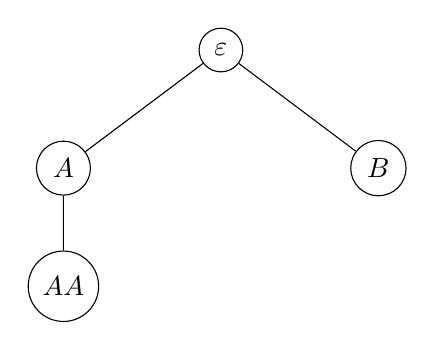
\begin{tikzpicture}[level/.style={sibling distance=40mm/#1}]
		\node [circle,draw] (epsilon){$\varepsilon$}
		child { node [circle,draw] (A) {$A$} 
			child { node[circle,draw](AA){$AA$}  }
		}
		child {node [circle,draw] (B) {$B$} }
		;
		
		\end{tikzpicture}
	\caption{Ejemplo de Modelo de predicción basado en un \emph{trie} con \texttt{LZ78}.}
	\label{fig:sim}
\end{figure}



Podemos ver que a menor cantidad de símbolos en la sesión generan un árbol de menor altura y menos nodos, cada nodo como se ha señalado en el capitulo 4 representa un visita a una sección en particular de la web de \emph{MSNBC}. Cuando un \emph{webaccess} posee  pocas secciones o páginas visitadas, la proyección de probabilidades de los posibles símbolos en el alfabeto hace que la probabilidad del siguiente acceso sea equiprobable dentro del los símbolos de nuestro diccionario, de lo anterior convergemos en que mayor es el entrenamiento mejor será la predicción.

Dado el evento $x$  a predecir que pertenece a una secuencia discreta, la probabilidad de $P( x| AB  ) = A $, es el resultado de esta sesión de entrenamiento, pero la probabilidad $P(x | AAB) $, es desconocida.  Si extendemos los símbolos de este nodo cada nodo hijo tendría un probabilidad de $ \dfrac{1}{\Sigma} = \dfrac{1}{17} = 0.0588 $ o bien sería  $\dfrac{1}{ |\sigma| }$, siendo $|\sigma|$ el total de símbolos que se encuentran en el alfabeto. 

Para corroborar este comportamiento haremos distintos experimentos en distintos volúmenes de datos, usaremos una validación cruzada para medir el \emph{Accuracy}, la cual será nuestra métrica a utilizar.

Con esto demostraremos que secuencias con menores cantidad de símbolos generar un tipo de ruido a la métrica  que afecta en su a nuestra exactitud esperada, cuando hacemos nuevos ciclos de evaluaciones sobre el mayor orden, por otra parte veremos como con una menor cantidad de sesiones de entrenamiento podemos lograr un \emph{Accuracy} bastante optimista.



\vspace{1cm}
\begin{enumerate}
	% Idea de experimento con disminución del tamaño del alfabeto
	\item\label{exp1} \textbf{Experimento con sesiones de usuarios con datos generados de forma sintética}
	
	Creamos un set de datos en el cual pudiesemos esperar valores conocidos. Además acotamos a un diccionario de solo tres element+os, el Accurracy obtenido es:
	
	
	
	\begin{figure}[h] 
		\centering
			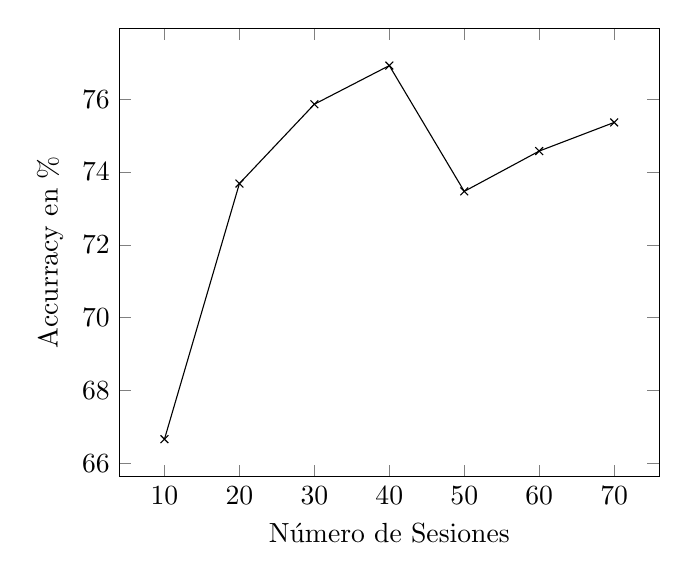
\begin{tikzpicture}
			\begin{axis}[
			xlabel= Número de Sesiones,
			ylabel=Accurracy en \% ]
			\addplot[color=black,mark=x] coordinates {
				(10, 66.6666666666666)
				(20, 73.6842105263157)
				(30, 75.8620689655172)
				(40, 76.9230769230769)
				(50, 73.469387755102)
				(60, 74.5762711864406)
				(70, 75.3623188405797)
			};
			\end{axis}
			\end{tikzpicture}	
		\caption{Experimento con set de datos sintéticos.}
		\label{fig:graph-exp1}
	\end{figure}
	

	
 
	
	En el gráfico \ref{fig:graph-exp1} usamos como mínimo 10 sesiones de las 80 de disponibles que se usaron par este experimento. Dado a que en este caso la cantidad de sesiones es bien reducida y cada símbolo posee una gran frecuencia existe mayor redundancia de datos y nuestro modelo se comporta como espera que lo haga un algoritmo de compresión de datos. Entre mayor es la cantidad de símbolos iguales
	que van entrenando al \emph{LZtrie}, hay una aglomeración de frecuencia en ciertos nodos, pero estos son minimizados por los niveles que genera al momento de la construcción del árbol.
	
	La tasa de frecuencia de un símbolo converge a predicciones de secuencias evaluadas que caen en el nodo con mejor probabilidad dado $\epsilon$ (Raíz del \emph{trie}).
	


	\newcommand{\slice}[4]{
		\pgfmathparse{0.5*#1+0.5*#2}
		\let\midangle\pgfmathresult
		
		% slice
		\draw[thick,fill=black!10] (0,0) -- (#1:1) arc (#1:#2:1) -- cycle;
		% outer label
		\node[label=\midangle:#4] at (\midangle:1) {};
		% inner label
		\pgfmathparse{min((#2-#1-10)/110*(-0.3),0)}
		\let\temp\pgfmathresult
		\pgfmathparse{max(\temp,-0.5) + 0.8}
		\let\innerpos\pgfmathresult
		\node at (\midangle:\innerpos) {#3};
	}
	
	\begin{center}
	\begin{tikzpicture}[scale=1.5]
	
	\newcounter{a}
	\newcounter{b}
	\foreach \p/\t in {61.5/page A, 35.9/page B, 12.8/type C }
	{
		\setcounter{a}{\value{b}}
		\addtocounter{b}{\p}
		\slice{\thea/100*360}
		{\theb/100*360}
		{\p\%}{\t}
	}
	
	\end{tikzpicture}
	\end{center}
	

	Tal como se puede ver en el gráfico anterior existe un gran probabilidad de que dado una secuencia de accesos después de $\epsilon$ la próxima sección a acceder sea la página A.
	Esto es adicionalmente es consistente a el tipo de set de datos que hemos ocupado ya que con esto podemos delimitar a que nuestro modelo al tener símbolos bastante frecuente no crea un trie desbalanceado, para este caso solo acota constantemente a un altura de 5 niveles y una variación mínima entre la exactitud, que posee el entrenamiento versus set de evaluaciones, incluso podemos solo podemos usar un entrenamiento de por lo menos 30 sesiones para predecir 50 sesiones con un Accurracy con un margen de error máximo de $10\%$ en el peor de los casos. 
	Lo anterior si lo comparamos con un evento aleatorio como resultado nos daría que nuestro modelo es bastante mejor que una predicción aleatoria, es decir $ 66.7\%  \geq 33\%$, siendo esta una comparativa optimista de que al menos nuestro modelo dado un set de datos artificial.
	
	
	
	
	\newpage
	\item \label{exp2} \textbf{Sesiones con menor redundancia y  largo variable }
		Validaremos ahora el comportamiento de nuestro modelo con datos reales con secuencias discretas distribuidas no uniformemente.
	
	
	
	\begin{figure}[h] 
		\centering
				\resizebox{0.6\textwidth}{!}{% <------ Don't forget this %
			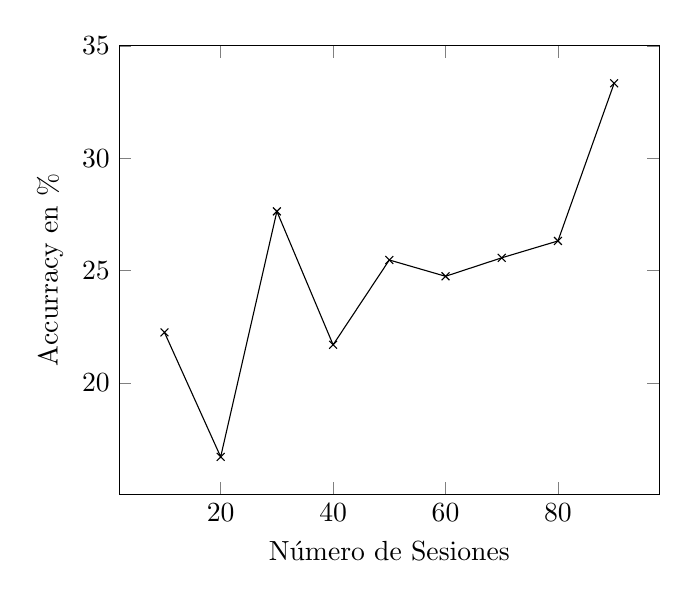
\begin{tikzpicture}
			\begin{axis}[
			xlabel= Número de Sesiones,
			ylabel=Accurracy en \% ]
			\addplot[color=black,mark=x] coordinates {
				(10, 22.2471910112359)
				(20, 16.7088607594936)
				(30, 27.6328502415459)
				(40, 21.6949152542372)
				(50, 25.469387755102)
				(60, 24.7435897435897)
				(70, 25.5665024630541)
				(80, 26.3157894736842)
				(90, 33.3333333333333)
			};
			\end{axis}
			\end{tikzpicture}
		}
		\caption{Experimento con secuencias de largo variable}
		\label{fig:experimento2}
	\end{figure}
	

	\begin{table}[h]
		\centering
		\label{tabla-exp-1}
		\begin{tabular}{ccccc}
			\textbf{pruebas}     & \textbf{entrenamiento} & \textbf{accuracy}    & \textbf{nodos}       & \textbf{niveles}     \\
			10                   & 90                     & 0,222471910112359    & 10                   & 5                    \\
			20                   & 80                     & 0,167088607594936    & 10                   & 5                    \\
			30                   & 70                     & 0,27632850241546     & 10                   & 5                    \\
			40                   & 60                     & 0,21694915254237     & 10                   & 5                    \\
			50                   & 50                     & 0,25469387755102     & 10                   & 5                    \\
			60                   & 40                     & 0,24743589743590   	 & 10                   & 5                    \\
			70                   & 30                     & 0,255665024630541    & 10                   & 5                    \\
			80                   & 20                     & 0,263157894736842    & 10                   & 5                    \\
			90                   & 10                     & 0,333333333333333    & 10                   & 5                    \\
			&                        &                      &                      &                      \\
			\multicolumn{1}{l}{} & \multicolumn{1}{l}{}   & \multicolumn{1}{l}{} & \multicolumn{1}{l}{} & \multicolumn{1}{l}{}
		\end{tabular}
		\caption{ Resumen de datos experimento 1}
	\end{table}



	\begin{table}[h] 	\label{tabl-exp-1-frec}
		\centering
		\resizebox{0.9\textwidth}{!}{% <------ Don't forget this %
	
		\begin{tabular}{lccccccccccccccccc}
			\textbf{símbolo}    & A  & B  & C  & D  & E & F  & G  & H  & I  & J  & K & L  & M  & N  & O & P & Q \\
			\textbf{frecuencia} & 64 & 19 & 18 & 29 & 4 & 36 & 20 & 65 & 20 & 11 & 4 & 15 & 42 & 31 & 2 & 0 & 0
		\end{tabular}
		
	}
		\caption{Tabla de frecuencia experimento 1}
	\end{table}


			
	En este caso si existe una menor redundancia a diferencia del experimento \ref{exp1} lo que produce que el modelo $M$ tenga un bajo rendimiento, aún así dada sigue siendo en el mejor de los casos seis veces mejor que la probabilidad aleatoria de predecir. En este experimento usamos un $|\sigma| =15$, por ende tenemos que dado nuestro modelo,
	\begin{equation}\label{expResult2}
		M( x | \mbox{90\% train}  ) = 33 \% \geq M( x | \mbox{random}  ) = 6.66 ,\% 
	\end{equation} como hemos visto en el experimento \ref{exp1} nuestro modelo sigue siendo válido en un escenario en que los datos se dispersan considerablemente. 
	Adicionalmente en este tipo de caso existe un comportamiento de nuestro modelo en el cual hace el mejor esfuerzo por mantener la \emph{compresibilidad} de los datos mayor o igual a la \emph{predictibilidad} del mismo, peor al tener mayor dispersión la altura para una cantidad similar de sesiones en \ref{exp1} sigue siendo $5$. Pero la cantidad de nodos sufre un gran incremento, podemos verlo en \ref{fig:exp-largo-variable-inf}
	
	
	
	\begin{figure}[h] 
		\centering
		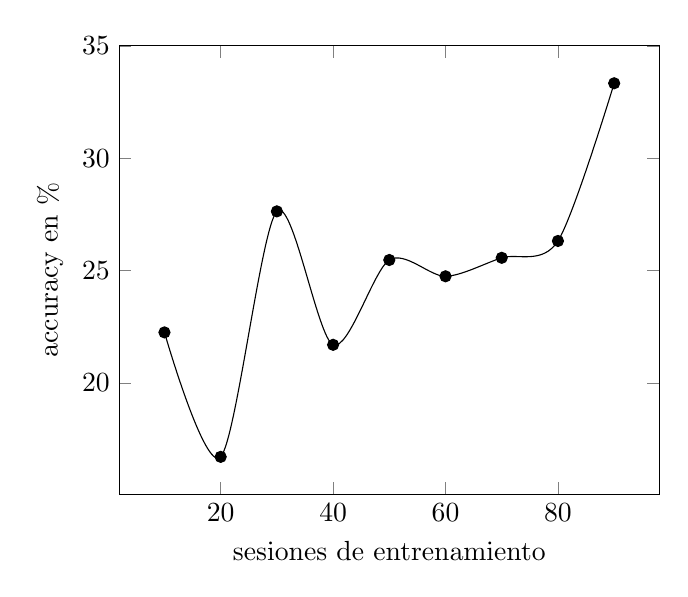
\begin{tikzpicture}
		\begin{axis}[
		xlabel=$\mbox{sesiones de entrenamiento}$,
		ylabel=$\mbox{accuracy en \%}$]
		\addplot[smooth,mark=*,black] plot coordinates {
			(10, 22.2471910112359)
			(20, 16.7088607594936)
			(30, 27.6328502415459)
			(40, 21.6949152542372)
			(50, 25.469387755102)
			(60, 24.7435897435897)
			(70, 25.5665024630541)
			(80, 26.3157894736842)
			(90, 33.3333333333333)
		};
		\end{axis}
		\end{tikzpicture}	
		
		\caption{Experimento con secuencias de largo variable inferiores y 100 sesiones}
		\label{fig:exp-largo-variable-inf}
	\end{figure}
	
	
	



	Acorde al gráfico \ref{fig:exp-largo-variable-inf} podemos señalar que al haber un incremento en la dispersión de datos y menor redundancia, el crecimiento de nuestro árbol será horizontal, ya que para tanto como hemos en este experimento y en (\label{expResult2}), la altura del nodo no tiene una relación directa a la redundancia ó dispersión, pero si a la cantidad de sesiones evaluadas. 
	
	Además, al mayor esfuerzo que hace el predictor por lograr mejores resultados se construyen mas nodos, por lo que el modelo LDC, deja de comprimir por satisfacer las condiciones de predictibilidad necesarias para seguir siendo válido.

	
	Iteramos una nueva evaluación con las mismas condiciones pero subiendo el volumen de datos de 100 a 1000. Con este buscaremos ver encontrar el mismo comportamiento a un mayor nivel de datos.
	


	
	
	\begin{figure}[t] 
		\centering
		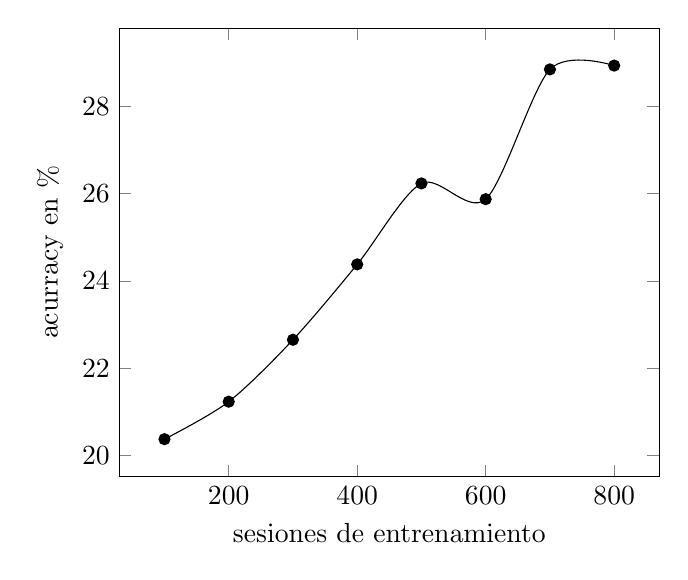
\begin{tikzpicture}
		\begin{axis}[
		xlabel=$\mbox{sesiones de entrenamiento}$,
		ylabel=$\mbox{acurracy en \%}$]
		\addplot[smooth,mark=*,black] plot coordinates {
			(100,  20.3715239154616)
			(200,  21.2302878598247)
			(300,  22.6490224129709)
			(400,  24.3752086811352)
			(500,  26.2308617234469)
			(600,  25.8692564745196)
			(700,  28.8423315814619)
			(800,  28.929431438127)
		};
		\end{axis}
		\end{tikzpicture}
		\caption{Experimento con secuencias de largo variable inferiore y 1000 sesiones}
		\label{fig:sim}
	\end{figure}
	
	El modelo sigue siendo válido al ir aumentando el volumen de datos bajo las mismas circunstancias. Incluso para ambos experimentos anteriores podemos sacar la relación que nuestro modelo posee una tasa de error de $\pm4\%$ al aumentar $100$ veces con respecto a la primera iteración de este escenario cuando se usa la  mayor cantidad de sesiones de entrenamiento posible.


	Otra particularidad que ha demostrado el modelo gracias a las propiedades de compresibilidad expuestas por  \emph{Lempel} \& \emph{Ziv}\cite{ZivLempel1977} es la minimización de niveles requeridos aún cuando la cantidad de nodos va creciendo.
	
	
	
	
	\begin{figure}[h] 
		\centering
			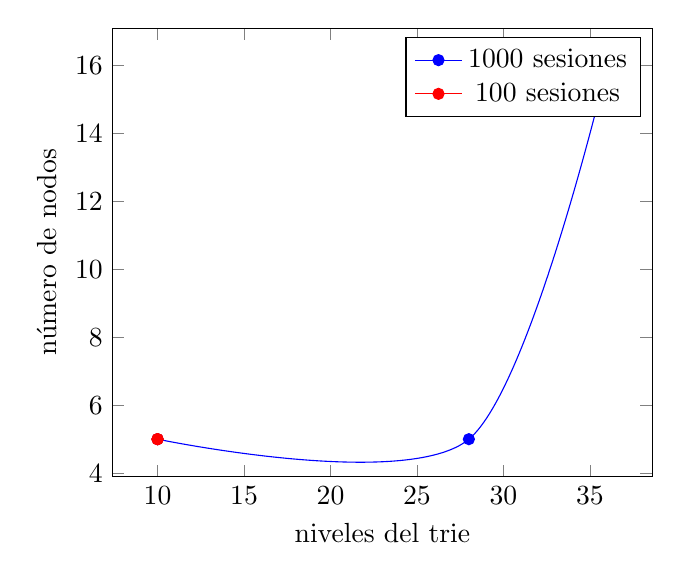
\begin{tikzpicture}
			\begin{axis}[
			xlabel=$\mbox{niveles del trie}$,
			ylabel=$\mbox{número de nodos}$]
			\addplot[smooth,mark=*,blue] plot coordinates {
				( 10 , 5 )
				( 28 , 5)
				( 36 , 16)
			};
			\addlegendentry{ 1000 sesiones }
			\addplot[smooth,mark=*,red] plot coordinates {
				( 10,5 )
				( 10,5 )
				( 10,5 )
			};
			\addlegendentry{ 100 sesiones }
			\end{axis}
			\end{tikzpicture}
		\caption{Gráfico comparativo para mismos niveles distinta cantidad de nodos.}
		\label{fig:sim}
	\end{figure}
	
	


	Como podemos ver en el comportamiento de inicio del modelo el criterio de partida en el escenario descrito es compartido por ambos experimentos.

	También dado a que no es uno de los escenarios más favorables para nuestro modelo predictivo, podríamos tener un diferencial en los tiempos de construcción del \emph{trie} respecto a la cantidad de nodos necesarios para el entrenamiento, 

	\begin{figure}[h] 
	\centering
	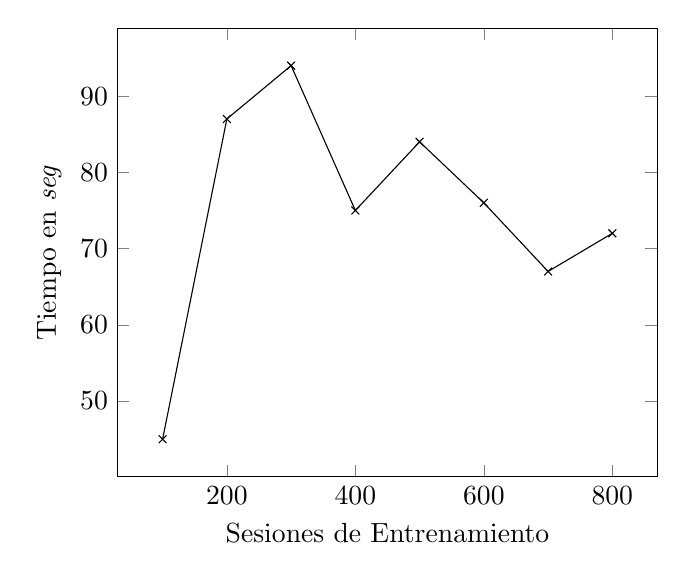
\begin{tikzpicture}
	\begin{axis}[
		xlabel= Sesiones de Entrenamiento ,
		ylabel= Tiempo en \emph{seg} ]
	\addplot[color=black,mark=x] coordinates {
			(100, 45 )
			(200, 87 )
			(300, 94 )
			(400, 75 )
			(500, 84 )
			(600, 76 )
			(700, 67)
			(800, 72 )
	};
	\end{axis}
	\end{tikzpicture}
		\caption{Gráfico de tiempo de construcción vs sesiones de entrenamiento}
	  \label{fig:sim}
	 \end{figure}	
	
	Como podemos ver en el gráfico anterior podemos buscar un dataset óptimo el cual puede encontrarse dentro del intervalo $ [ 300,400 ]$ sesiones de usuario, equivalente a la mejores resultados de \emph{Accurracy} y menor cantidad de secuencias de entrenamiento.


	\item \label{exp3}	
	\textbf{Sesiones con tamaño de secuencia constante}
	En este experimentos queremos lograr el mismo comportamiento que tuvimos en el experimento [\ref{exp1}]. Haciendo un filtrado simple de los \emph{webaccess log } que hemos estado analizando podemos llegar a mejores valores que las predicciones de resultado aleatorio.





	\begin{figure}[h] 
		\centering
			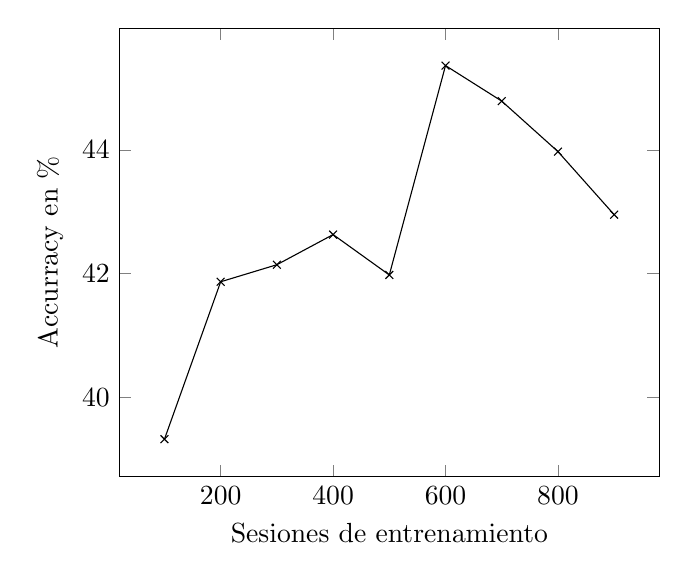
\begin{tikzpicture}
			\begin{axis}[
			xlabel=Sesiones de entrenamiento,
			ylabel=Accurracy en \% ]
			\addplot[color=black,mark=x] coordinates {
				(100, 39.3259176863181 )
				(200, 41.8698372966207 )
				(300, 42.1454458750596 )
				(400, 42.6323038397328 )
				(500, 41.9799599198396 )
				(600, 45.3634085213033 )
				(700, 44.7892976588628)
				(800, 43.9736180904522 )
				(900, 42.9539842873176 )
			};
			\end{axis}
			\end{tikzpicture}
		\caption{Gráfico de Accuracy vs sesiones de largo constante}
		\label{fig:sim}
	\end{figure}



	
	La cantidad total de sesiones usadas fueron $1000$ y las cuales como en el gráfico anterior se señala a mayor cantidad entrenamiento existe al menos un punto de la curva que se vuelve un máximo.


	Seguido a esto podemos ver el tiempo de construcción del \emph{Trie} que nuestro modelo demora en generar:
	
	
	
	\begin{figure}[h] 
		\centering
		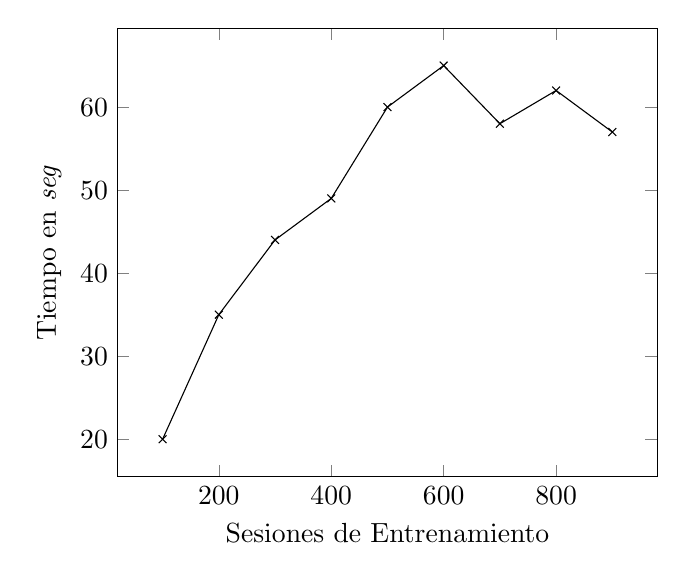
\begin{tikzpicture}
		\begin{axis}[
		xlabel= Sesiones de Entrenamiento ,
		ylabel=Tiempo en \emph{seg} ]
		\addplot[color=black,mark=x] coordinates {
			(100, 20)
			(200, 35)
			(300, 44)
			(400, 49)
			(500, 60)
			(600, 65)
			(700, 58)
			(800, 62)
			(900, 57 )
		};
		\end{axis}
		\end{tikzpicture}
		\caption{Gráfico de Tiempo vs sesiones de largo constante}
		\label{fig:sim}
	\end{figure}
	
	

	Al igual que en el gráfico anterior podemos ver que existe al menos una mínima cantidad sesiones las cuales generar un rendimiento sobre las evaluaciones a realizar. 
	

	\item \label{exp4} \textbf{Secuencias de accesos con limite inferior 100 símbolos }
	Este experimento busca validar las condiciones necesarias que debe tener una secuencia de entrada para que el algoritmo \texttt{LDC} pueda optimizar al momento de ser construido para una predicción \emph{online}, dado esto utilizaremos sesiones largas que entreguen redundancia en los accesos que permita al modelo de navegación ser más comprimido sin perder una métrica considerable para funcionar, según lo anterior realizamos las siguientes iteraciones con las particiones de data que cumplen: 
	
	\begin{figure}[h] 
		\centering
		\resizebox{.7\textwidth}{!}{
		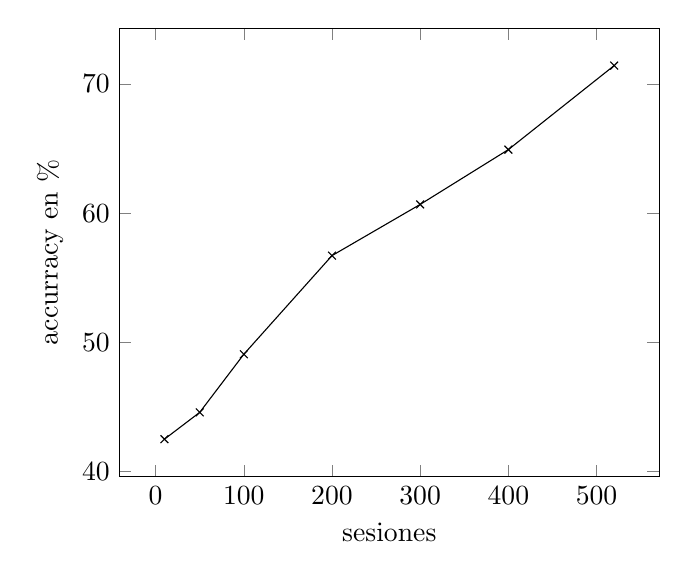
\begin{tikzpicture}
		\begin{axis}[
			xlabel= sesiones,
			ylabel=accurracy en \% ]
		\addplot[color=black,mark=x] coordinates {
			(10 ,  42.5190839694656 )
			(50 ,  44.595041322314 )
	 		(100 , 49.089861751152 )
	 		(200 , 56.7230538922155 )
	 		(300 , 60.6837606837608 )
	 		(400 , 64.9253731343282 )
	 		(520 , 71.4285714285715 )			
		};
		\end{axis}
		\end{tikzpicture}
		}
		\caption{Gráfico de Accuracy para sesiones mayores de 100 símbolos}
		\label{fig:sim}
	\end{figure}
	
	
	Sean la sesiones de entrenamiento de tamaño $T$, con un valor  $T(100) = 49 \% $ sobre un set de evaluación $E(100) = 900 \mbox{ sesiones}$ , nuestro modelo propuesto al igual que en el experimento \ref{exp1}, entrega un punto mínimo el cual al menos da un $50\%$ de acierto sobre el total de $535$ sesiones de usuarios, con una secuencia mínima de $100$ símbolos. Planteado de otra forma, sólo con el $20\%$ del total de datos de entrenamiento nuestro motor de predicción ya alcanza un \emph{Accurracy} que es mucho mejor que un predictor aleatorio sobre el alfabeto del experimento. Siendo este valor bastante optimista acorde a los puntos óptimos del predictor que use la menor cantidad de recursos.
	
	
	\begin{figure}[h] \label{fig:sim}
	\centering
		\resizebox{.7\textwidth}{!}{
		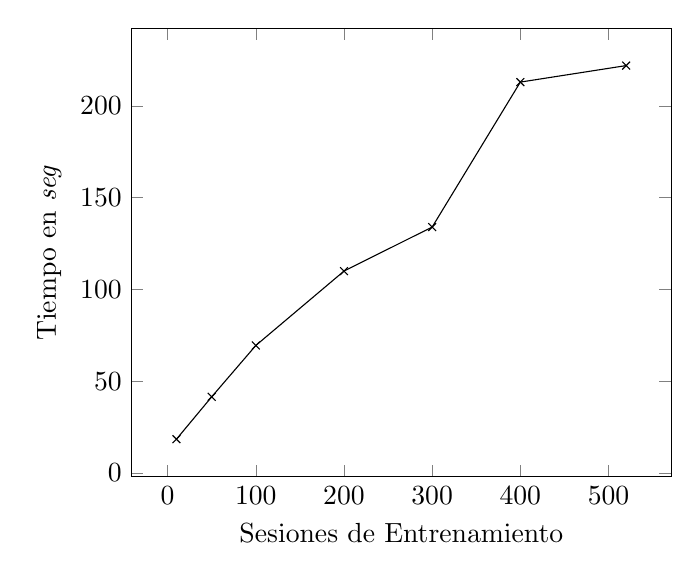
\begin{tikzpicture}
		\begin{axis}[
		xlabel= Sesiones de Entrenamiento ,
		ylabel=Tiempo en \emph{seg} ]
		\addplot[color=black,mark=x] coordinates {
			(10 ,  18.4)
			(50 ,  41.5)
			(100 , 69.46)
			(200 , 110)
			(300 , 134)
			(400 , 213)
			(520 , 222)	
		};
		\end{axis}
		\end{tikzpicture}
		}
		\caption{Gráfico de tiempo vs sesiones de entrenamiento\\ para sesiones mayores de 100 símbolos}
		
	\end{figure}


\begin{table}[h]
	\centering
	\caption{Tabla resumen experimento 4}
	\label{my-label}
	\begin{tabular}{ccccc}
		\textbf{pruebas} & \textbf{entrenamiento} & \textbf{accuracy} & \textbf{nodos} & \textbf{niveles} \\
		990              & 10                     & 0,21422649140546  & 38             & 5                \\
		950              & 50                     & 0,3104531085353   & 95             & 5                \\
		900              & 100                    & 0,393259176863181 & 132            & 5                \\
		800              & 200                    & 0,418698372966207 & 181            & 5                \\
		700              & 300                    & 0,421454458750596 & 208            & 5                \\
		600              & 400                    & 0,426323038397328 & 241            & 5                \\
		500              & 500                    & 0,419799599198396 & 264            & 5                \\
		400              & 600                    & 0,453634085213033 & 288            & 5                \\
		300              & 700                    & 0,407892976588628 & 308            & 5                \\
		200              & 800                    & 0,439736180904522 & 326            & 5                \\
		100              & 900                    & 0,429539842873176 & 349            & 5               
	\end{tabular}
\end{table}

\begin{table}[]
	\centering

	\label{my-label}
	\resizebox{0.9\textwidth}{!}{
	\begin{tabular}{lccccccccccccccccc}
		\textbf{símbolo}    & A    & B    & C   & D   & E   & F   & G   & H    & I   & J   & K   & L   & M   & N   & O   & P  & Q  \\
		\textbf{frecuencia} & 2162 & 1044 & 269 & 757 & 225 & 815 & 681 & 1207 & 370 & 278 & 233 & 453 & 502 & 860 & 102 & 10 & 32
	\end{tabular}
	}
	\caption{Tabla resumen de simbolos y frecuencia para experimento 4}
\end{table}

	Congruente con lo anterior podemos ver que sin tener un margen de error superior a la porción de datos seleccionado logramos un latencia de consulta predictiva en línea de alrededor de 70 \emph{seg}, el cual para ser implementado y consumido como ya se había mencionado antes como un algoritmo predictivo como servicio \emph{REST}, esta dentro del promedio aceptable.

	\begin{figure}[h] 
		\centering
		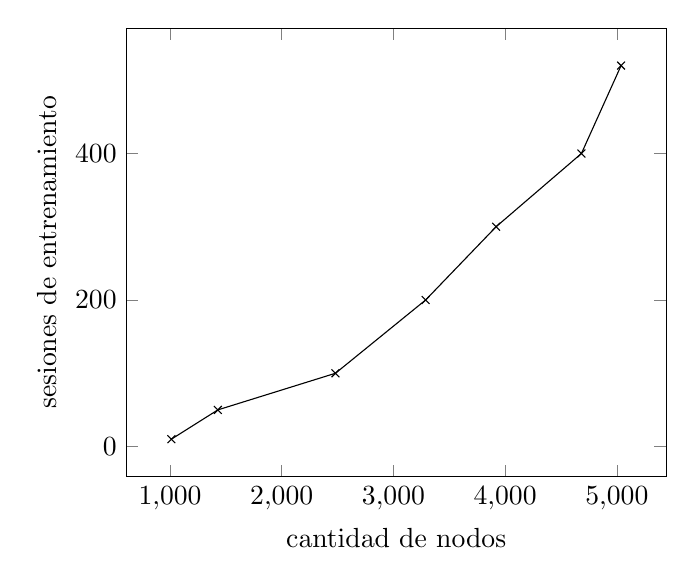
\begin{tikzpicture}
		\begin{axis}[
			xlabel= cantidad de nodos,
			ylabel= sesiones de entrenamiento  ]
		\addplot[color=black,mark=x] coordinates {
			(1012,10 )
			(1428,50 )
			(2481,100 )
			(3288,200 )
			(3919,300 )
			(4683,400 )
			(5038,520 )	
		};
		\end{axis}
		\end{tikzpicture}	
		\caption{Gráfico de cantidad de nodos vs sesiones de entrenamiento para sesiones mayores de 100 símbolos}
	  \label{fig:sim}
	\end{figure}


	Otro de los puntos  considerado aceptable, es que dado un set de entrenamiento $T(100)$, solo necesitaremos menos de la mitad de nodos que se requieren para llegar a un valor de predicción bueno, a diferencia de una partición de entrenamiento que requiere más del $90\%$ de nodos del total del set de datos.\\
	

	
	\begin{figure}[h] 
		\centering
			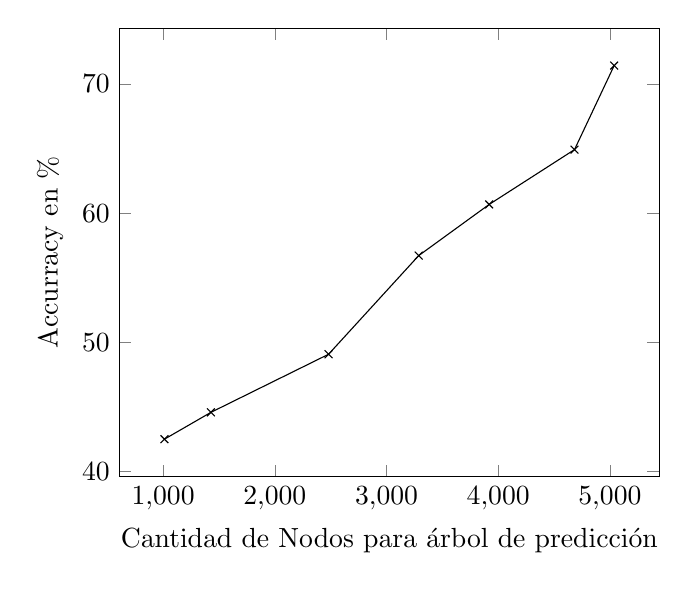
\begin{tikzpicture}
			\begin{axis}[
			xlabel=Cantidad de Nodos para árbol de predicción,
			ylabel=Accurracy en \%  ]
			\addplot[color=black,mark=x] coordinates {
				(1012,42.5190839694656 )
				(1428,44.595041322314 )
				(2481,49.089861751152 )
				(3288,56.7230538922155 )
				(3919,60.6837606837608 )
				(4683,64.9253731343282 )
				(5038,71.4285714285715 )	
			};	
			\end{axis}
			\end{tikzpicture}	
			\caption{Gráfico de cantidad de nodos vs Accuracy para sesiones mayor de 100 símbolos}
		\label{fig:sim}
	\end{figure}



	Finalmente podemos señalar que la tasa de \emph{Accuracy}, aún  subiendo al doble la cantidad de nodos para construir un \emph{trie} de \texttt{LZ78}, con mayor información  para predecir alcanza un rendimiento aceptable respecto de la compresión realizada. De todas maneras también se cumple que la cantidad de nodos del entrenamiento es directamente proporcional a la métrica seleccionada.


	\item \label{exp5}	
	\textbf{Sesiones con menos de 5 \emph{webaccess} para generar el \emph{trie}}
		Hacemos una validación cruzada para una muestra de data de 906130 sesiones de usuarios para probar como se comporta con cross validation.
	
	
	
	\begin{figure}[h] 
		\centering
			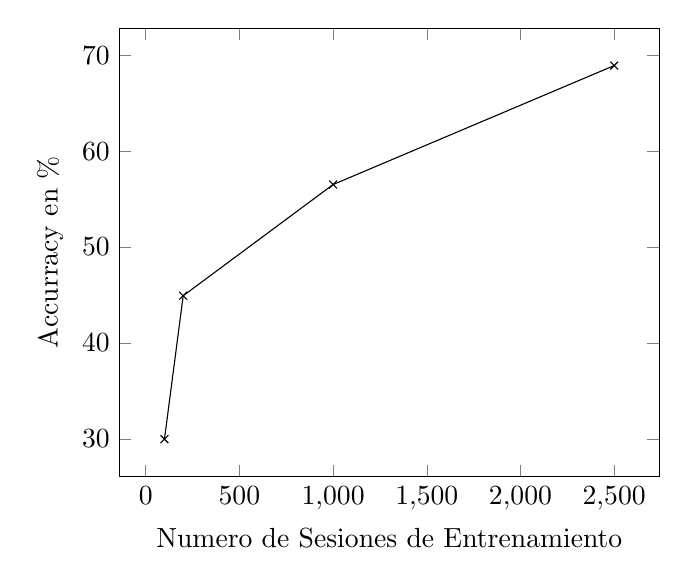
\begin{tikzpicture}
			\begin{axis}[
			xlabel= Numero de Sesiones de Entrenamiento,
			ylabel=Accurracy en \% ]
			\addplot[color=black,mark=x] coordinates {
				(100, 29.9674371114825)
				(200, 44.9237667712101)
				(1000, 56.519572924979)
				(2500, 68.9237667712101)	
			};
			\end{axis}
			\end{tikzpicture}
		\caption{Gráfico de Accuracy vs sesiones de entrenamiento para una cota superior de 5 símbolos}
		\label{fig:sim}
	\end{figure}	
	
	
	\item \label{exp6} 
	\textbf{Detección de Ruido en secuencias de acceso}
	
	Al modelar una navegación de usuario mediante un \emph{trie} basado en un algoritmo como \texttt{LZ78}, adoptamos un enfoque basado en la frecuencia por lo cual si realizamos experimentos para poder encontrar ruido veremos que que son secuencias de acceso comunes y estas no dan relevancia o aportan a la exactitud ó precisión del algoritmo.
	
	Sea la secuencia $\{A,A,A,A,A,A,A,A,A,A,A,A \}$ a la cual llamaremos secuencia $R$, si $A$ es representado por el \emph{home} ó página de inicio, esto da a interpretación que existe un usuario en su sesión $R$ que se encuentra accediendo constantemente a esta sección. Podemos señalar que esta es una sesión ruidosa si:
	
	\begin{equation}
		P( x | AAAAAAA)= A ,	
	\end{equation} pero siendo la sesión $R$ de tamaño = $12$, en el siguiente acceso tendremos una probabilidad equiprobable dentro de las secciones en nuestro alfabeto, la cual generará un probabilidad de éxito ''falso positivo''.
	
	En el siguiente experimento veremos como se comporta nuestro modelo dado entradas \emph{Ruidosas}. Además se mostrará como el árbol suele perder su balance a medida que va creciendo los niveles de altura. 
	
	
	
	Por otro lado teniendo la noción de como es el funcionamiento de un servidor \texttt{IIS}, y al ser una página con un gran número de visitas, podemos señalar que los datos proporcionados no son totalmente representativos de usuarios reales, ya que la web al bien indexada en los buscadores existen un cantidad indeterminada de \emph{Crawlers} ó \emph{Bots} que están constantemente generando accesos tanto para almacenar en caché páginas o generando accesos automatizados a ciertos secciones sin ser datos representativo. Dejamos como discusión que algoritmo se podría implementar para detección de estos patrones por las ramas que hemos generado para la detección de \emph{bots} o \emph{robots}.
	
	
	
	
	 
	
	%	\item  Dataset uniformes de largo acotado inferiormente y volumenes de alto tamaño.
\end{enumerate}








 



	% \begin{forest} 
	% 	[VP
	% 	[DP]
	% 	[V’
	% 	[V]
	% 	[DP]
	% 	]
	% 	]
	% \end{forest}



	% \begin{tikzpicture}[level/.style={sibling distance=60mm/#1}]
	% \node [circle,draw] (z){$n$}
	% child {node [circle,draw] (a) {$\frac{n}{2}$}
	% 	child {node [circle,draw] (b) {$\frac{n}{2^2}$}
	% 		child {node {$\vdots$}
	% 			child {node [circle,draw] (d) {$\frac{n}{2^k}$}}
	% 			child {node [circle,draw] (e) {$\frac{n}{2^k}$}}
	% 		} 
	% 		child {node {$\vdots$}}
	% 	}
	% 	child {node [circle,draw] (g) {$\frac{n}{2^2}$}
	% 		child {node {$\vdots$}}
	% 		child {node {$\vdots$}}
	% 	}
	% }
	% child {node [circle,draw] (j) {$\frac{n}{2}$}
	% 	child {node [circle,draw] (k) {$\frac{n}{2^2}$}
	% 		child {node {$\vdots$}}
	% 		child {node {$\vdots$}}
	% 	}
	% 	child {node [circle,draw] (l) {$\frac{n}{2^2}$}
	% 		child {node {$\vdots$}}
	% 		child {node (c){$\vdots$}
	% 			child {node [circle,draw] (o) {$\frac{n}{2^k}$}}
	% 			child {node [circle,draw] (p) {$\frac{n}{2^k}$}
	% 				child [grow=right] {node (q) {$=$} edge from parent[draw=none]
	% 					child [grow=right] {node (q) {$O_{k = \lg n}(n)$} edge from parent[draw=none]
	% 						child [grow=up] {node (r) {$\vdots$} edge from parent[draw=none]
	% 							child [grow=up] {node (s) {$O_2(n)$} edge from parent[draw=none]
	% 								child [grow=up] {node (t) {$O_1(n)$} edge from parent[draw=none]
	% 									child [grow=up] {node (u) {$O_0(n)$} edge from parent[draw=none]}
	% 								}
	% 							}
	% 						}
	% 						child [grow=down] {node (v) {$O(n \cdot \lg n)$}edge from parent[draw=none]}
	% 					}
	% 				}
	% 			}
	% 		}
	% 	}
	% };
	% \path (a) -- (j) node [midway] {+};
	% \path (b) -- (g) node [midway] {+};
	% \path (k) -- (l) node [midway] {+};
	% \path (k) -- (g) node [midway] {+};
	% \path (d) -- (e) node [midway] {+};
	% \path (o) -- (p) node [midway] {+};
	% \path (o) -- (e) node (x) [midway] {$\cdots$}
	% child [grow=down] {
	% 	node (y) {$O\left(\displaystyle\sum_{i = 0}^k 2^i \cdot \frac{n}{2^i}\right)$}
	% 	edge from parent[draw=none]
	% };
	% \path (q) -- (r) node [midway] {+};
	% \path (s) -- (r) node [midway] {+};
	% \path (s) -- (t) node [midway] {+};
	% \path (s) -- (l) node [midway] {=};
	% \path (t) -- (u) node [midway] {+};
	% \path (z) -- (u) node [midway] {=};
	% \path (j) -- (t) node [midway] {=};
	% \path (y) -- (x) node [midway] {$\Downarrow$};
	% \path (v) -- (y)
	% node (w) [midway] {$O\left(\displaystyle\sum_{i = 0}^k n\right) = O(k \cdot n)$};
	% \path (q) -- (v) node [midway] {=};
	% \path (e) -- (x) node [midway] {+};
	% \path (o) -- (x) node [midway] {+};
	% \path (y) -- (w) node [midway] {$=$};
	% \path (v) -- (w) node [midway] {$\Leftrightarrow$};
	% \path (r) -- (c) node [midway] {$\cdots$};
	% \end{tikzpicture}



%Las conclusiones son deducidas logicamen- te de los resultados obtenidos y de la interpretacionpresen- tada, ademas estan conectadas al marco teorico.
%Las conclusiones muestran el logro de los ob jetivos.
%Se presentan proyec- ciones validas y valio- sas a partir del traba- jo realizado.
%Se detallan claramen- te las limitaciones del traba jo realizado.




 


 
%%%%%%%%
%%%%%%%%


 

El orden de como se ingresan las sesiones afecta directamente proporcional a la construcción del modelo \emph{trie},  por lo cual es un factor  \emph{FIFO} al momento de crear, lo primero que lee es lo primero que entrena por lo cual se debiese tener un criterio para ordenar los \emph{webaccess} antes de poder pasarlos al entrenador, que implica antes de la construcción.

El modelo propuesto, básicamente es un compresor el cual no toma decisiones, una posible mejora sería implementar un árbol de decisiones con algún criterio para decidir que entrenar y que no, estos árboles pueden estar dentro del \emph{trie} para
poder elegir secuencias optimo acorde a los criterios históricos, así podría darse el caso de ser un compresor--predictor  \emph{mas inteligente}.



















\vspace{2cm}
\section{Conclusiones y Contribuciones}\label{ch:conlusion-contrib-all}
	\input{contrib-conlusion}






\newpage
\subsection{Trabajos Futuro}

Esta memoria forma parte del plan de continuidad en el postgrado de la Escuela de Ingeniería Informática y telecomunicaciones, por lo cual se desea profundizar este trabajo en las discusiones realizadas. Los temas deseados por abarcar:

\begin{itemize}

\item Crear un estudio comparativo con Modelos de \emph{Machine Learning} como (\emph{RNN}) Redes Neuronales, Reglas de Asociación, \emph{Deep Learning} y algoritmo de tipo \emph{Frequent Pattern Growth}.

\item Técnicas para mejorar el modelo de predicción 
\item Mejorar la implementación de \texttt{LZ78}, realizado con lenguaje funcional y objetos(\emph{Scala}) y hacer una comparación de rendimientos contra implementaciones clásicas en lenguajes de más bajo nivel (\texttt{C++}).


\item Crear técnicas como la usada por Claude \etal~\cite{Claude2014}, para crear representaciones eficientes en función de este modelo predictivo.


\item Investigar los factores teóricos y técnicos para poder mejorar la exactitud de la predicción.

\item Ambiciosamente a realizar un estudio comparativo para encontrar puntos en común de estas áreas de la ciencia de la computación, se desea crear un nuevo algoritmo basado en la familia de \emph{Lempel Ziv}, el cual pueda tener un complemento para la selección de sesiones antes ser ingresadas en el modelo de navegación predictivo. 


	
\end{itemize}	






 












% Iniciamos el resto de secciones adicionales al contenido: referencias y apendices
\backmatter

%%Se presenta una revision bibliografica acertada, actual, y exhaustiva (se consulta toda la literatura relevante).


%Presenta y redacta los objetivos, el trabajo realizado, y la validacion de manera deta-llada. Presenta discusiones detalladas, articuladas, claras, y un buen uso del lengua je tecnico.


% Bibliografía
% El estilo por defecto es IEEE Transactions
\bibliographystyle{ieeetr}
\bibliography{IEEEabrv,referencias}


% Simbología y glosario
% Utilice un paquete para generar símbolos y glosarios.
% Por ejemplo: nomencl (http://texdoc.net/pkg/nomencl)
% Anexos
\appendix
% Aca se incluyen los archivos con el texto de los anexos
\chapter{Anexos técnicos}
\label{ch:anexo-a}


\section{Uso de linea de Comando Prediction.IO}


La interación con \emph{PIO} es a través de una interface de linea de comando, esta sigue el siguiente formato de uso:

 

\begin{lstlisting}[frame=single,basicstyle=\ttfamily\tiny,]
  pio <command> [options] <args>...
\end{lstlisting}



En caso de tener duda usted al igual que los comandos de bash puede ejecutar

\begin{lstlisting}[frame=single,basicstyle=\ttfamily\tiny,]
pio help <command> 
\end{lstlisting}, para ver mas detalles de cada detalle de los comandos disponibles.


Los comandos de PredictionIO se pueden separar en tres categorías:

\begin{itemize}
	\item \textbf{help} Muestra un resumen del uso  \emph{pio help <command>} para leer sobre un sub comando
	
	\item \textbf{Version} Muestra la version instalada de PredictionIO
	
	
	\item \textbf{Status} Muesta la ruta de instalación y el estatus de ejecución de sistema, como también sus dependencias
	
\end{itemize}

Comandos del servidor de eventos



\begin{itemize}
	\item \textbf{app} Muestra un resumen del uso  \emph{pio help <command>} para leer sobre un sub comando
	
	\item \textbf{Version} Muestra la version instalada de PredictionIO
	
	
	\item \textbf{app }  Administra todas las aplicaciones que usa el servidor de eventos
	\item \textbf{pio app data-delete <name> } Borra toda la data contenida por una aplicación específica
	\item \textbf{pio app delete <name> }  Borra una aplicación completa
	\item \textbf{eventserver }  Lanza el servidor de eventos
	\item \textbf{ --ip <value> } Une la IP seleccionada, el valor por defecto es \emph{localhost}
	\item \textbf{access\_key} Administra todas las llaves de acceso al servidor de eventos ó app
	
\end{itemize}


\section {Comandos del Motor de Predicción}

Es requerido que estos comandos se ejecuten desde la misma carpeta que contiene el proyecto ó aplicación desplegada.

Las opciones  --debug y --verbose  muestran información detallada sobre los conectoes de las aplicaciones complementarias a las que esta compuesta PredictionIO

\begin{itemize}
	\item \textbf{build} Construye y compila el proyecto completo desde la carpeta fuente, tiene un flag adicional \emph{-- clean}, para una compilación limpia.

	\item \textbf{train} Ejecuta el entrenamiento declarado en el motor 

	\item \textbf{deploy} Despliega el motor para ser usado meiante REST como Algoritmo como Servicio. Si no existe ninguna nueva instancia  desplegada, por defecto usará la última creada.
	
\end{itemize}


\newpage
\section{Configuraciones para hacer correr IntelliJ con Apache SPARK y Prediction.IO 0.94}

\begin{lstlisting}[frame=single,basicstyle=\ttfamily\tiny,]
Main class: io.prediction.workflow.CreateWorkflow

VM options: -Dspark.master=local -Dlog4j.configuration=file:/Users/jguzman/PredictionIO/conf/log4j.properties


Program arguments: --engine-id dummy --engine-version dummy --engine-variant engine.json


io.prediction.workflow.CreateWorkflow
-Dspark.master=local -Dlog4j.configuration=file:/Users/jguzman/PredictionIO/conf/log4j.properties -Dorg.xerial.snappy.lib.name=libsnappyjava.jnilib 
--engine-id dummy --engine-version dummy --engine-variant engine.json



SPARK_HOME=/Users/jguzman/PredictionIO/vendors/spark-1.4.1/bin
PIO_FS_BASEDIR=/Users/jguzman/.pio_store
PIO_FS_ENGINESDIR=/Users/jguzman/.pio_store/engines
PIO_FS_TMPDIR=/Users/jguzman/.pio_store/tmp
PIO_STORAGE_REPOSITORIES_METADATA_NAME=pio_meta
PIO_STORAGE_REPOSITORIES_METADATA_SOURCE=ELASTICSEARCH
PIO_STORAGE_REPOSITORIES_MODELDATA_NAME=pio_model
PIO_STORAGE_REPOSITORIES_MODELDATA_SOURCE=LOCALFS
PIO_STORAGE_REPOSITORIES_APPDATA_NAME=pio_appdata
PIO_STORAGE_REPOSITORIES_APPDATA_SOURCE=ELASTICSEARCH
PIO_STORAGE_REPOSITORIES_EVENTDATA_NAME=pio_event
PIO_STORAGE_REPOSITORIES_EVENTDATA_SOURCE=HBASE
PIO_STORAGE_SOURCES_ELASTICSEARCH_TYPE=elasticsearch
PIO_STORAGE_SOURCES_ELASTICSEARCH_HOSTS=localhost
PIO_STORAGE_SOURCES_ELASTICSEARCH_PORTS=9300
PIO_STORAGE_SOURCES_LOCALFS_TYPE=localfs
PIO_STORAGE_SOURCES_LOCALFS_HOSTS=/Users/jguzman/.pio_store/models
PIO_STORAGE_SOURCES_LOCALFS_PORTS=0
PIO_STORAGE_SOURCES_HBASE_TYPE=hbase
PIO_STORAGE_SOURCES_HBASE_HOSTS=0
PIO_STORAGE_SOURCES_HBASE_PORTS=0


Main class: io.prediction.workflow.CreateServer
Program Arguments: --engineInstanceId **replace_with_the_id_from_pio_train**




Try -- for more information.
Usage: pio train [--batch <value>] [--skip-sanity-check]
                 [--stop-after-read] [--stop-after-prepare]
                 [--engine-factory <value>] [--engine-params-key <value>]
                 [--scratch-uri <value>]
                 [common options...]

Kick off a training using an engine (variant) to produce an engine instance.
This command will pass all pass-through arguments to its underlying spark-submit
command.

  --batch <value>
      Batch label of the run.
  --skip-sanity-check
      Disable all data sanity check. Useful for speeding up training in
      production.
  --stop-after-read
      Stop the training process after DataSource.read(). Useful for debugging.
  --stop-after-prepare
      Stop the training process after Preparator.prepare(). Useful for
      debugging.
  --engine-factory
      Override engine factory class.
  --engine-params-key
      Retrieve engine parameters programmatically from the engine factory class.
  --scratch-uri
      URI of the working scratch space. Specify this when you want to have all
      necessary files transferred to a remote location. You will usually want to
      specify this when you use --deploy-mode cluster.

\end{lstlisting}

\vspace{1cm}


\section {Llamadas al Servidor de Machine Learning mediante curl }


\begin{lstlisting}

curl -H "Content-Type: application/json"  -d '{"webaccess" : "AC","num" : 10}' http://52.33.180.212:8000/queries.json



\end{lstlisting}



\section{Python SDK para PredictionIO}

Para hacer uso de estos scripts en python es necesario tener instalado el package de prediction para python sdk.

Si se tiene pip instalado correctamente se puede utilizar

\begin{verbatim}
pip install predictionio
\end{verbatim}
ó
\begin{verbatim}
$ easy_install predictionio
\end{verbatim}


Es recomendable tener acceso sudo para evitar problemas con permisos al momento de usar \emph{pip} o \emph{easy\_install} {(ie. sudo pip install predictionio)}.




El siguiente script, permite hacer una sola consulta la cual puede ser ejecutada desde el \emph{cli} de python ó llamando directamente al archivo ejecutable. ( {python test.py})

\begin{lstlisting}[frame=single,basicstyle=\ttfamily\tiny,]
import predictionio

engine_client = predictionio.EngineClient(url="http://localhost:8000")

print engine_client.send_query({"webaccess": "A", "num": 10})
\end{lstlisting}



\newpage
A diferencia del script explicado anteriomente este permite enviar secuencias desde la terminal \emph{cli}, la cual puede seguir en ejecución hasta que el usuario finalice el proceso.

\begin{lstlisting}[frame=single,basicstyle=\ttfamily\tiny,]
"""
Send sample query to prediction engine
"""

import predictionio
import readline

engine_client = predictionio.EngineClient(url="http://localhost:8000")
while True:
    word = raw_input('Enter a Sequences or a single page to predict the next user webaccess: \n')
    print engine_client.send_query({"webaccess": word, "num": 10})

\end{lstlisting}





\section{Programa C++ para hacer splits dentro del Dataset}
Programa para poder pasar la data de msnbc a una representación de símbolos.

\begin{lstlisting}[frame=single,basicstyle=\ttfamily\tiny,]
#include <iostream>     // cout
#include <fstream>      // ifstream
#include <sstream>
#include <algorithm>
#include <string>
#include <cmath>
#include <cstdio>
#include <vector>
#include <map>
#include <iterator>

using namespace std;

/** 
  alias lseq = g++ -std=c++11 letterSequences.cpp -o letterSequences 
  ./letterSequences

% Different categories found in input file:

frontpage news tech local opinion on-air misc weather msn-news health living business msn-sports sports summary bbs travel
**/

 
int main()
{
   map<string, int> mapCategories;

  
   // Inserting data in map
  mapCategories.insert(make_pair("frontpage", 1));
    mapCategories.insert(make_pair("news",    2));
    mapCategories.insert(make_pair("tech",    3));
    mapCategories.insert(make_pair("local",   4));
    mapCategories.insert(make_pair("opinion",   5));
    mapCategories.insert(make_pair("on-air",  6));
    mapCategories.insert(make_pair("misc",    7));
    mapCategories.insert(make_pair("weather",   8));
    mapCategories.insert(make_pair("msn-news",  9));
    mapCategories.insert(make_pair("health",  10));
    mapCategories.insert(make_pair("living",  11));
    mapCategories.insert(make_pair("business",  12));
    mapCategories.insert(make_pair("msn-sports",13));
    mapCategories.insert(make_pair("sports",  14));
    mapCategories.insert(make_pair("summary",   15));
    mapCategories.insert(make_pair("bbs",     16));
    mapCategories.insert(make_pair("travel",  17));
    

   vector<char> alphabet = { 'A','B','C','D','E','F','G',
                'H','I','J','K','L','M','N','O',
                'P','Q','R','S','T','U','V','W',
                'X','Y','Z'};

   // Iterate through all elements in map
   map<string, int>::iterator it = mapCategories.begin();

   ifstream  fin("msnbc990928.seq");
   string    file_line;
   int fold = 0 ;

   while(getline(fin, file_line)){

    string    buf; // Have a buffer string
    stringstream  ss(file_line); // Insert the string into a stream
    vector<string> tokens; // Create vector to hold our words
    
    while (ss >> buf) tokens.push_back(buf);

    if( tokens.size() < 6 ){
      ++fold;
      for (int i = 0; i < tokens.size(); ++i){
        string tmp = tokens.at(i); 
        cout << alphabet.at( stoi(tmp) - 1) << " ";
      }cout<< endl;

    }

    //this value is for make the size of the folds of data
    if( fold == 1000000 ) break;

   }
    return 0;
}
\end{lstlisting}















\end{document}